\chapter{Results} \label{ch:results}

\textcolor{purple}{Redo the old graphs. Two lines instead of four in scatter plots.}

%In this chapter, we first evaluate our algorithm for random model generation and analyze structural biases of the real case studies.
In this chapter, we present first the technical details of our experimental setup.
Next, we analyze the structural biases of the real case studies and compare them to the structural biases of randomly generated models we have created.
Furthermore, we evaluate our algorithm for random generation in terms of scalability and runtime performance.
Then, we compare algorithm performance on the real case studies as well as our randomly generated models and investigate which model features influence the performance of the algorithms.

%Regarding runtime a lot of stuff may change. Iterations wont change as long as we use the same deterministic algorithms, so its a more stable metric.

%Various studies we have made, knit into a nice purple string and story. Here might appear:
%Maybe it would also be cool to show preformance differences in real case studies in comparison to the randomly generated models and make conclusions Ideally:

\section{Experimental setup}
First, we discuss the details of our experimental setup.
Various algorithms we consider were already implemented in PRISM-games~\cite{prismgames3}.
We extended PRISM-games by the algorithms $\LPSI$, $\SISI$, and $\TOPAlg$.
Moreover, for $\TOPAlg$ and $\SISI$, we added linear equation solving with Gurobi version 9\footnote{https://www.gurobi.com/}, which we used with an academic license.
For $\LPSI$, we use Gurobi version 9 too.
Our code is available in the GitHub repository \url{https://github.com/ga67vib/Algorithms-For-Stochastic-Games}.

\subsubsection*{Technical details}
We conducted the experiments on a server with 64 GB of RAM and a 3.60GHz Intel CPU running Manjaro Linux. %Intel (R) Xeon(R) W-2123 CPU.
We always use a precision of $\varepsilon=10^{-6}$. 
The timeout was set to 15 minutes, and the memory limit was 6 GB for all models except for the set of large models (see Subsection \ref{subsec:largeModels}),
where the timeout was set to 30 minutes and the memory limit to 36 GB.

\subsection{Case studies} \label{subsec:casestudies}
We consider case studies from four different sources: 

(i) real case studies, of which all but "teamform" (\cite{teamform}) were already used in~\cite{gandalf}, and which are mainly from the PRISM benchmark suite~\cite{PRISMben}.
For a detailed description of the real case studies, see \cite[Appendix C.1]{gandalf}.
We omit models that are already solved by pre-computations.
With variations of the model parameters, we obtain 18 models.

(ii) several handcrafted corner case models: Haddad-Monmege (an adversarial model for value iteration from~\cite{haddadmonmege}), BigMec (a single big MEC), and MulMec (a long chain of many small MECs), the latter two both being from~\cite{gandalf}.

(iii) 300 randomly generated models generated by Algorithm \ref{alg:randomRandom} and our additional guidelines from Subsection \ref{sec:guidelines}.
For the exact parameters we have used to generate our models See Appendix \ref{sec:GenParams}. Without models solved by pre-computations, we obtain 284 models.

(iv) large models (models with at least 100,000 states) with a structure similar to the RandomTree guideline (see Section \ref{sec:guidelinesSubsec}) and generated at runtime with our alternative to handcrafting as described in Section \ref{sec:configs}.
The difference to models generated with the RandomTree guideline is that every inner tree node has three deterministic actions, and only the leaves have probabilistic actions that lead into either the next SCC, the target, the sink, or the root of the tree.
The models have at least 100,000 states and at most 5 million states. For each size, there is one model where the whole state space is strongly connected, and another one where there the state space is divided into five equally large SCCs.

\subsection{Plot overview} \label{subsec:plots}
We provide a short description of each type of plot we use in this chapter:
\subsubsection*{Box plots} \label{plot:boxplot}
A box plot provides an overview of the spread and skewness of the model features of our model sets.
See Table \ref{tab:modelFeatures} for an overview of all model features we track and an explanation of the abbreviations.
The orange line marks the median of a feature in all models, and the green triangle marks the
average. The bounds of the boxes mark the 25 and 75 percentile, and the extended lines 
mark the last data point included in the interquartile range times the factor 1.5. Dots outside the whiskers represent
outliers that differ significantly from the rest of the dataset.
The plots are grouped by and colored into the following categories:
\begin{itemize}
    \item Green outlines are for properties related to states. 
    \item Blue outlines are for properties related to actions. 
    \item Cyan outlines are for properties related to transitions.
    \item Red outlines are for properties related to MECs.
    \item Orange outlines are for properties related to SECs. 
\end{itemize}

\subsubsection*{Line plots for accumulated algorithm performance} \label{plot:starplot}
To provide a general overview performance of all stochastic game algorithms, we use line plots.
The plot depicts the number of solved benchmarks (x-axis) and the time it took to solve them (y-axis). 
For each algorithm, the benchmarks are sorted ascending by verification time. A line stops when no further benchmarks could be solved.
Intuitively, the further to the bottom right a plot is, the better; where going right (solving benchmarks) is more relevant.
The legend on the right is sorted by the performance of the algorithms in descending order.
Note that this plot has to be interpreted with care, as it greatly depends on the selection of benchmarks.

\subsubsection*{Scatter plots for algorithm performance} \label{plot:performanceScatter}
While line plots compare models solved and accumulated performance, scatter plots allow us to compare algorithm performance model by model.
Each point in the graph is a model. The x-axis marks the time/iterations one algorithm requires to solve a model, and the y-axis marks the respective time/iterations of the compared algorithms.
If a point is below the diagonal, the algorithm on the x-axis required more time to solve it than the corresponding algorithm on the y-axis and vice versa.
The two lines next to the diagonal mark the case where one algorithm was twice as fast as the other.

\subsubsection*{1-dimensional scatter plots} \label{plot:1Dscatter}
We use 1-dimensional scatter plots to visualize whether structural features favor one event over another.
In some cases, we want to analyze how two sets of events $\mathbf{A}, \mathbf{B}$ correlate to model features. 
Usually, we use $\mathbf{B}$ as the complement to $\mathbf{A}$.
An example for such a pair is: 
$\mathbf{A}$ contains all the models where algorithm X was 1.5 times faster than algorithm Y.
$\mathbf{B}$ contains all the models where algorithm X was not 1.5 times faster than algorithm Y.
We study the properties of the models in $\mathbf{A}$ and the properties of the models in $\mathbf{B}$ 
by scattering the feature values of models in $\mathbf{A}$ against scattering feature values of models in $\mathbf{B}$. 
When using this plot, we try to identify whether models in $\mathbf{A}$ distribute
differently along the spectrum of feature values than $\mathbf{B}$.

\section{Model analysis results}
In this section, we use our analysis tools to investigate structural biases in the real case studies and in our randomly generated models.
First, we want to learn about the feature distribution of the real case studies we have. 
For this, we use a box plot for each feature in Figure \ref{fig:Real_FeatureDistribution}.
\begin{figure}[h!]
    \centering
    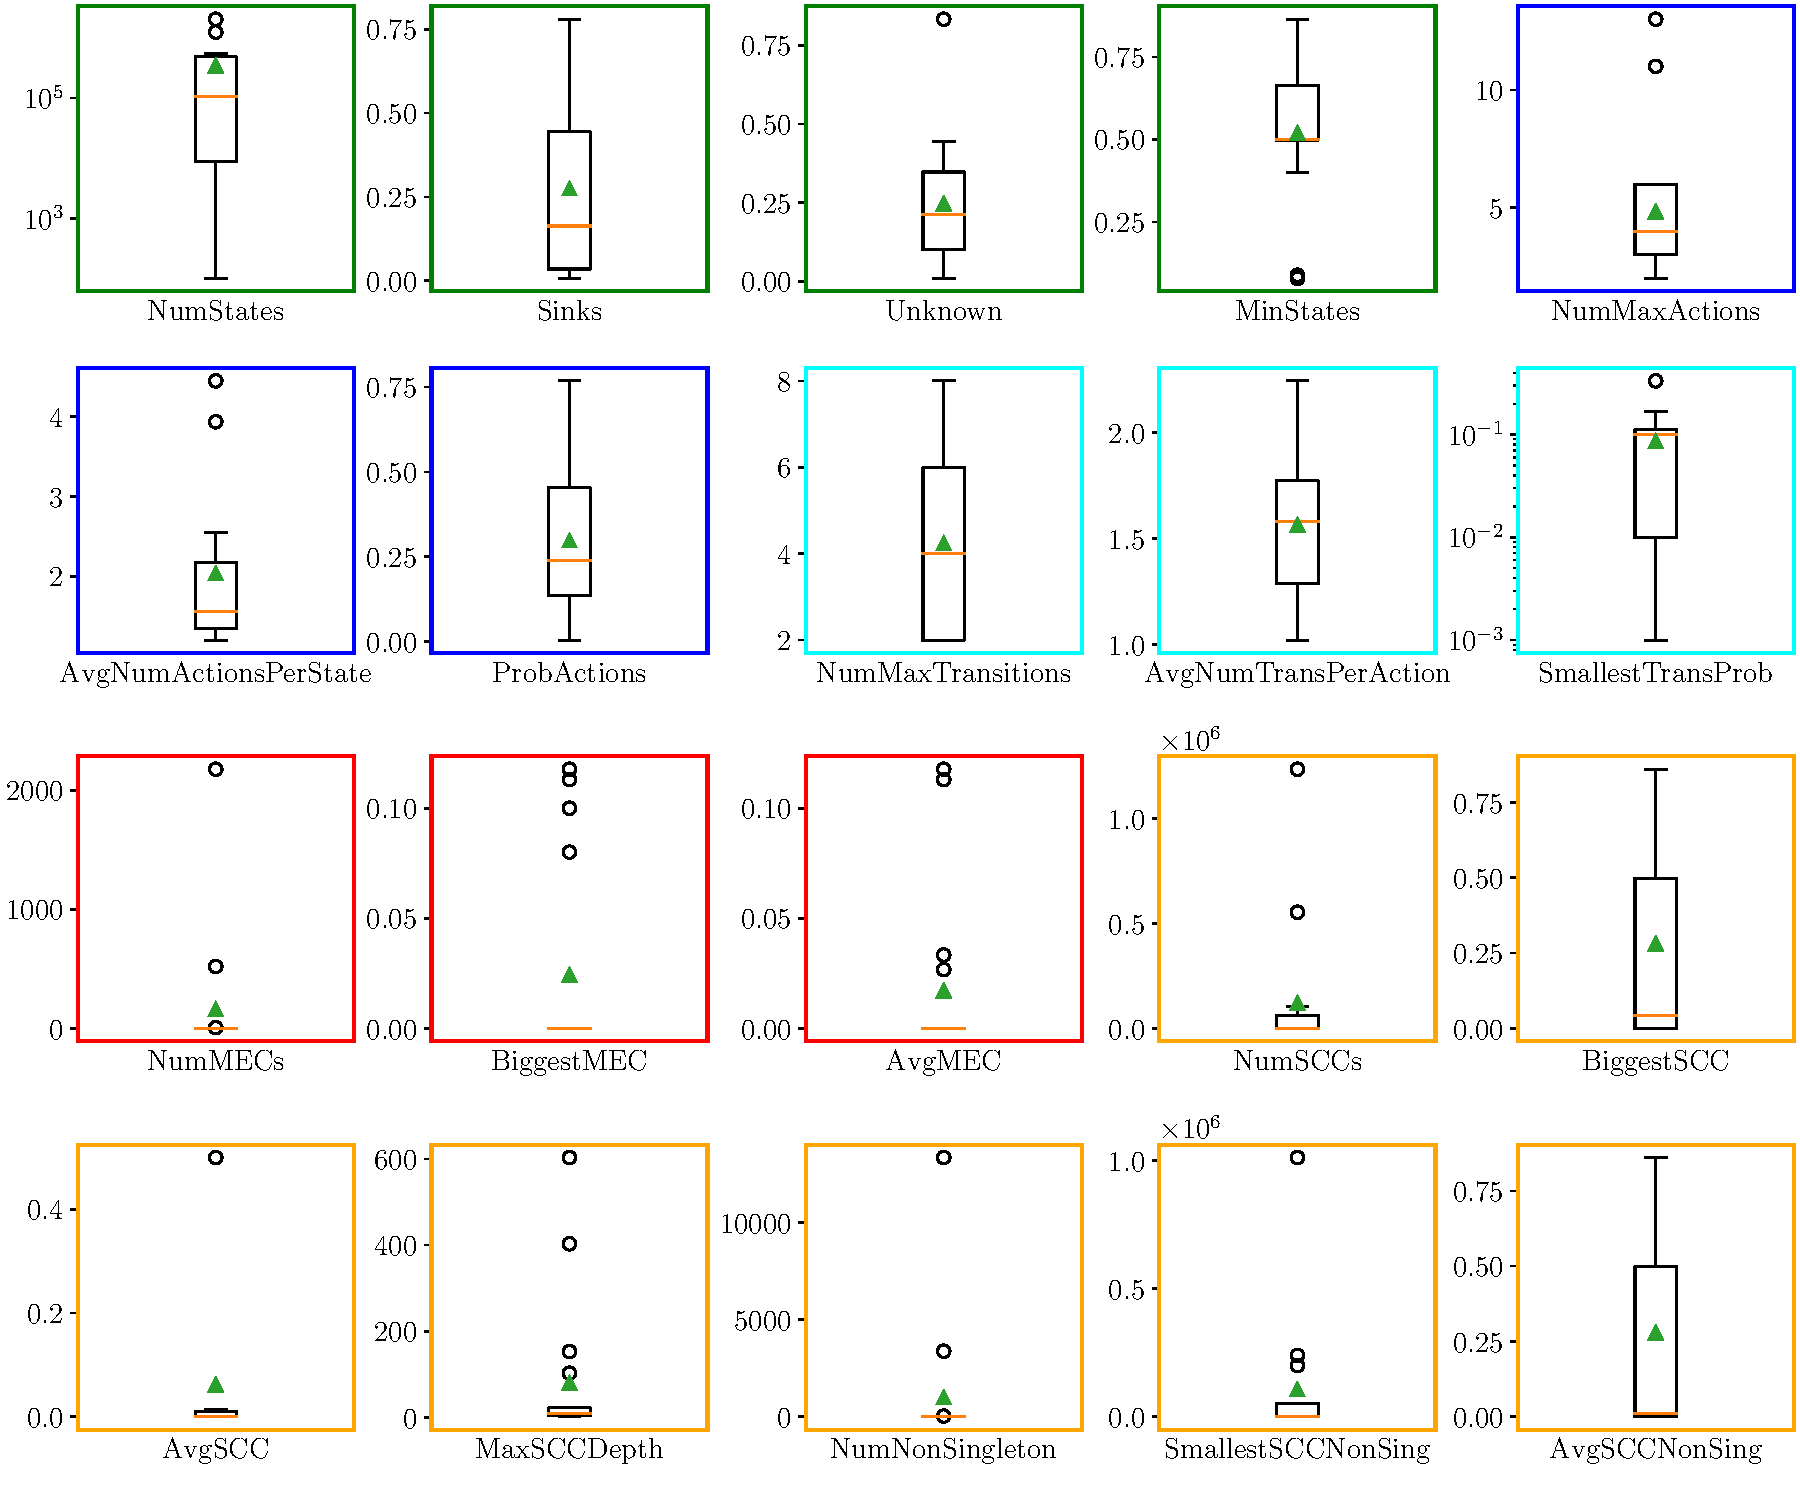
\includegraphics[width=1\textwidth]{figures/Real_FeatureDistribution.pdf}
    \caption[Feature Distribution of the case studies]{
        A Box plot of the feature distribution of the real case studies.
        The description of how to read the plot is provided in Section \ref{plot:boxplot}.
    }
    \label{fig:Real_FeatureDistribution}
\end{figure}
The box plots provide the following insights:
\begin{itemize} \label{insights:realDistribution}
    \item On average models have 2 actions per state and 1.5 transitions per action (see AvgNumActionsPerState and AvgNumTransPerAction).
    \item The plot for NumUnknown shows that usually at least 50\%, and on average 80\% of the states of the models are trivial, and their value is computed during pre-computation with simple graph algorithms. 
    \item Generally, the Maximizer controls as many states as the Minimizer.
    \item The plot for NumProbActions indicates that usually, around 70 to 85\% of all actions are deterministic.
    \item Most models do not contain end components as NumMECs shows.
\end{itemize}

By furthermore inspecting the maximal and minimal occurring values of each feature we obtain that the smallest occurring transition probability is 0.001.

We also use the information to draw conclusions about which structural cases do not appear in the real case studies. 
None of the models contain these cases:
\begin{itemize}
    \item Models with numerous actions per state,
    \item models with numerous transitions per action, or
    \item models with very small transition probabilities.
\end{itemize}
\FloatBarrier
However, this does not say that these properties are necessarily unrealistic. Instead, they did not appear in problems people have modeled so far.
After analyzing the real case studies, we now investigate the biases of the randomly generated models we have generated with Algorithm \ref{alg:randomRandom}.
Figure \ref{fig:Random_FeatureDistribution} contains the box plots for our randomly generated models. 
\begin{figure}[h!]
    \centering
    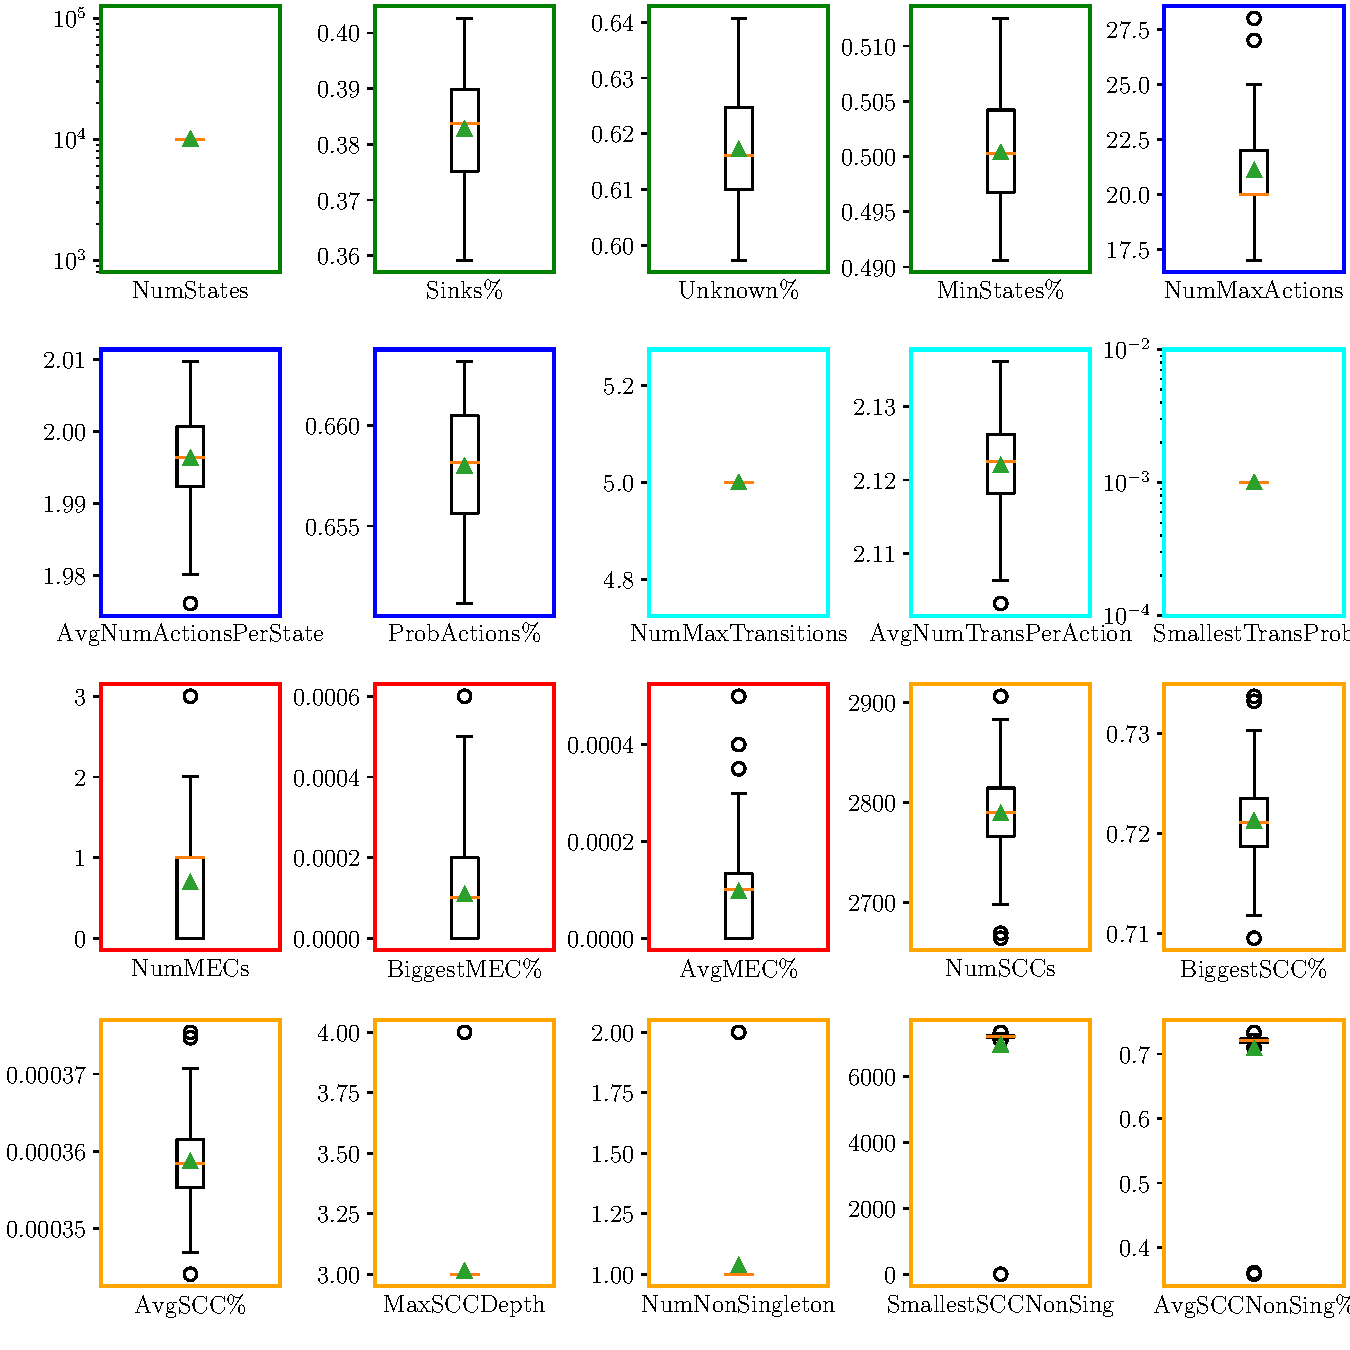
\includegraphics[width=1\textwidth]{figures/RandomRandom_FeatureDistribution.pdf}
    \caption[Feature Distribution of randomly generated models]{
        A Box plot of the feature Distribution of models generated randomly with Algorithm \ref{alg:randomRandom}. The description of how to read the plot is provided in Section \ref{plot:boxplot}.
        For each plot, 100 data points are used.
        %The evaluation of the plot is located in Section \ref{insights:randomRandom}.
    }
    \label{fig:Random_FeatureDistribution}
\end{figure}
 
The biases we read from this plot are:
\begin{itemize} \label{insights:randomRandom}
    \item Unknown\% indicates that on average, 38.5\% of the state-values are obtained during pre-computation. Sinks\% shows that almost all known states are sinks.
    \item With the chosen parameters, our algorithm generates models with 2 actions per state on average and 2 transitions per action on average (see AvgNumActionsPerState and AvgNumTransPerAction).     
     However, our parameters allow us to change the number of actions and transitions per state.
    \item NumNonSingleton shows that in almost all cases, there is only one strongly connected component.
        This is because we uniformly randomize where a transition may lead. Thus, it is likely that big SCCs are formed. 
        If necessary, the RandomSCC guideline can control the size of the SCCs.
    \item NumMECs indicates that there is usually either one MEC or none at all. Also, the MECs tend to have very few states (usually no more than 2).
    However, there are parameter configurations that favor generation of larger MECs. For example, setting the parameters in such a way that the actions are deterministic
    and adding one or multiple actions to every state in the backward procedure of Algorithm \ref{alg:randomRandom} creates models with a high tendency of forming few MECs that usually contain almost the whole state-space.
    Nevertheless, without providing a specific guideline, we have very limited control over the number and size of the MECs.
    \item Our random generation algorithm introduces a bias towards various properties like the number of SCCs or the average number of transitions per action.
    While on average models have only two actions, the maximal number of actions a state has is usually between 20 and 22 as NumMaxActions indicates.
    When analyzing the number of actions in relation to the state index, states with many actions always have low indices.
\end{itemize}

When comparing the feature distributions of the real case studies and the distributions of the models generated by Algorithm \ref{alg:randomRandom},
they have similar biases for many features. Both benchmarks tend to have few big SCCs, few actions per state, and few transitions per action.
However, we are not restricted to creating models similar to the current case studies. The number of actions and transitions can be adjusted by parameters,
and the how SCCs are formed can be influenced by guidelines, as described in Section \ref{sec:guidelines}.
\FloatBarrier

To demonstrate this, we present in Figure \ref{fig:RandomSCC_FeatureDistributions} the feature distribution of a set of models we have created by using the RandomSCC guideline.
Here, we constrain that every SCC should have 1000 to 2000 states. For the exact generation parameters, see Section \ref{sec:GenParams}.
Figure \ref{fig:Random_FeatureDistribution} contains the box plots for our randomly generated models.
\begin{figure}[h!]
    \centering
    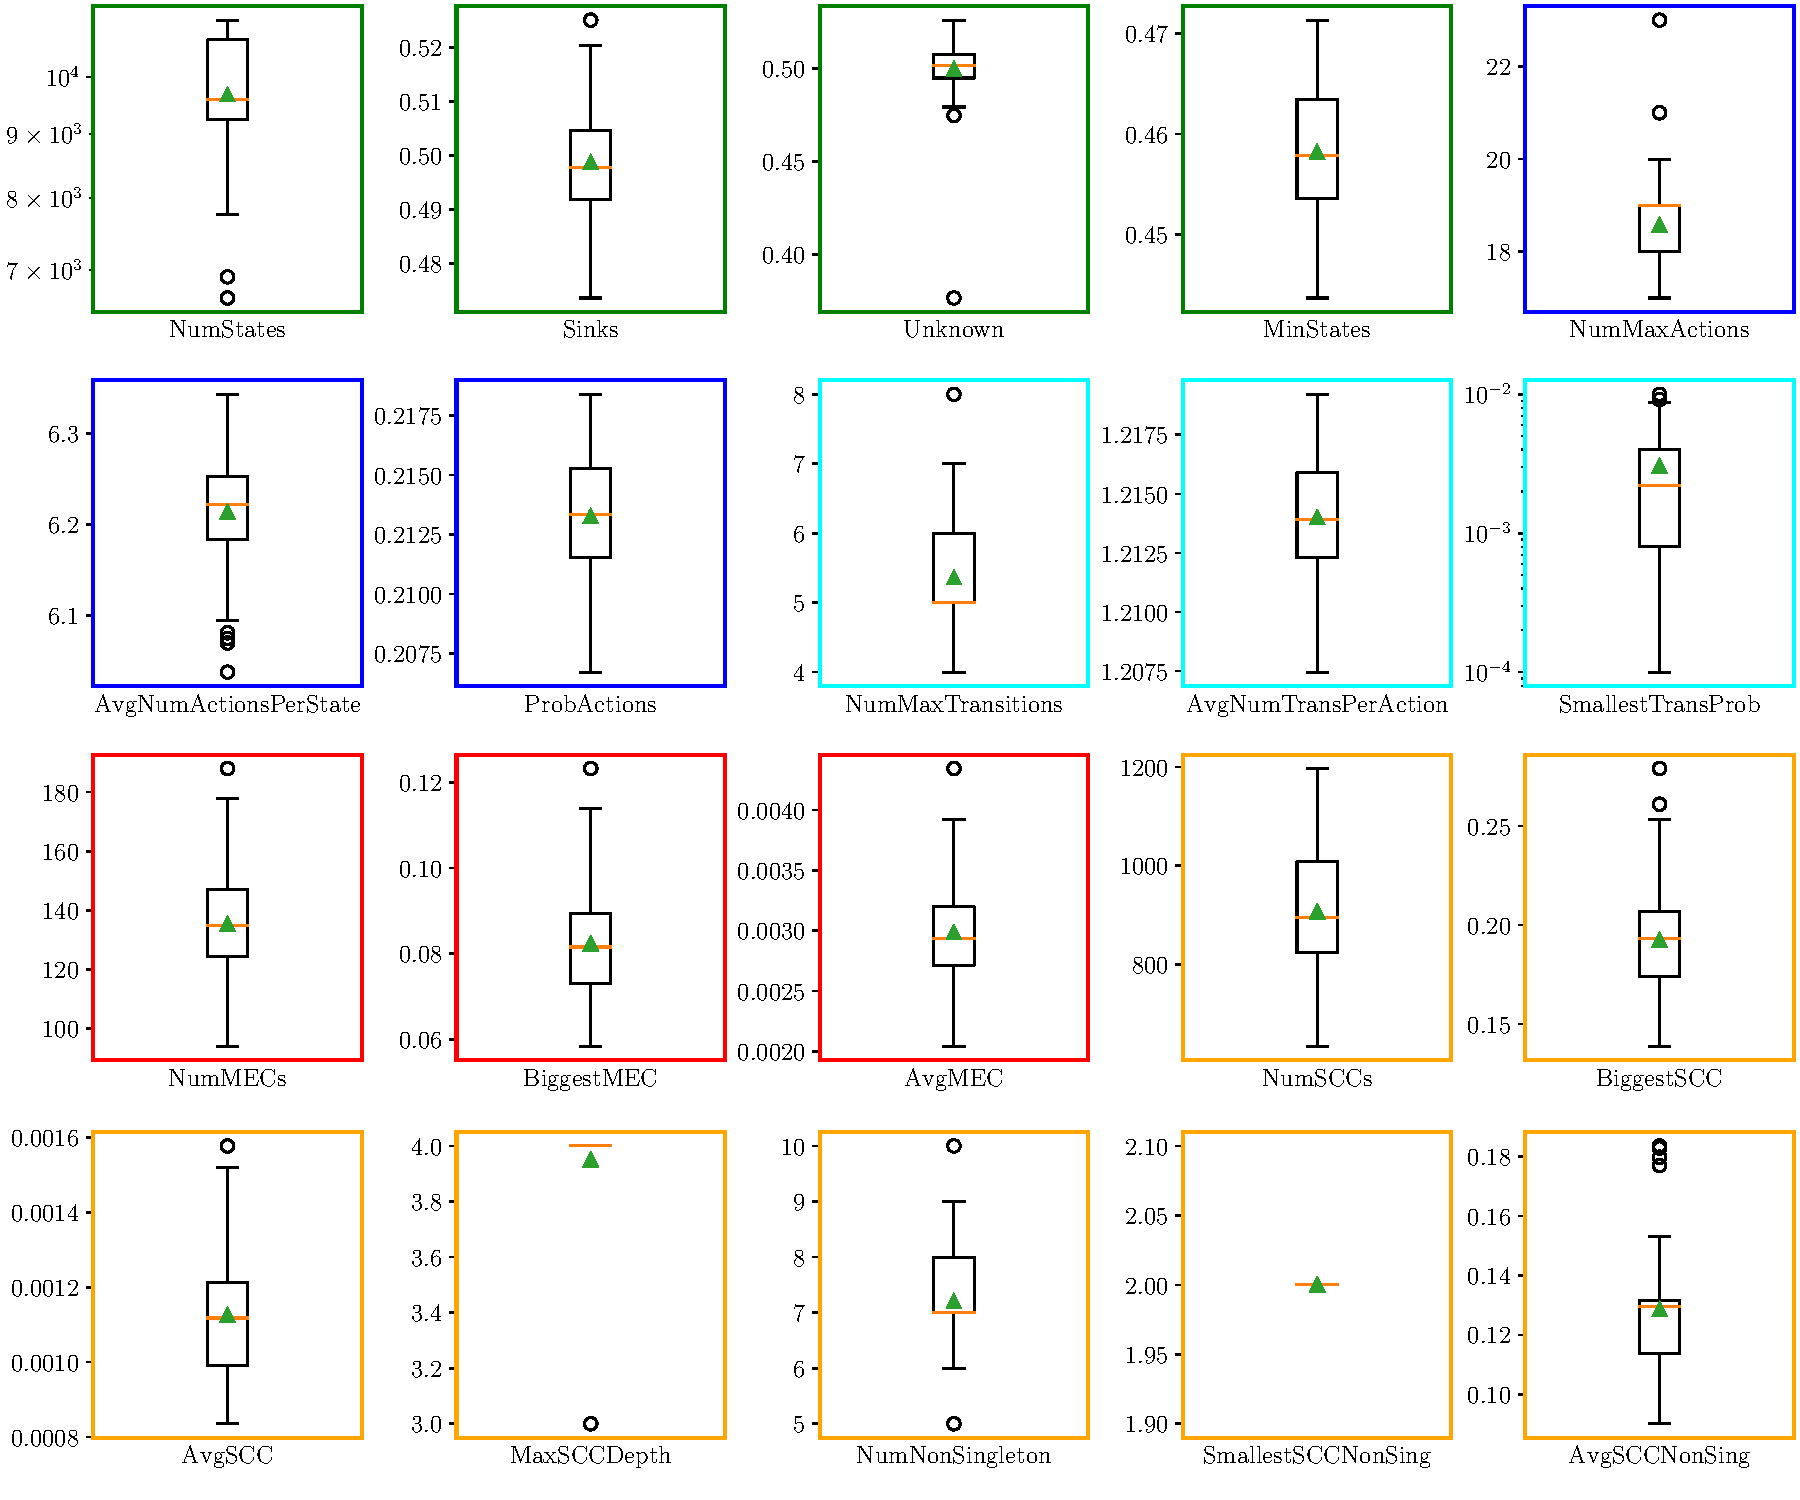
\includegraphics[width=1\textwidth]{figures/RandomSCC_FeatureDistribution.pdf}
    \caption[Feature Distribution of randomly generated models with the RandomSCC guideline]{
        Feature Distribution of randomly generated models by applying the RandomSCC guideline. The description of how to read the plot is provided in Section \ref{plot:boxplot}.
        For each plot, 100 data points are used.
        %The evaluation of the plot is located in Section \ref{insights:sccDistribution}.
    }
    \label{fig:RandomSCC_FeatureDistributions}
\end{figure}
\FloatBarrier

\label{insights:sccDistribution}
Clearly, the guideline allows us to control the size of the SCCs. No SCC has more than 2000 states, which is the upper bound we provided.
Also, MaxActions is not as biased as in Algorithm \ref{alg:randomRandom}. However, this is only due to the SCCs being smaller.
If every SCC had size 10000, the bias similar to random generation without guideline.

\section{Evaluating our random model generation}
Now that we have evaluated the models we generated, we evaluate the random generation algorithm itself in this section.
We investigate the capabilities of generating large models and the required time to generate a model. Furthermore, we discuss difficulties 
we encountered in generating non-trivial models with our implementation as described in Chapters \ref{ch:randomGen} and \ref{ch:implementedRandomGen}.

\subsection{Generating large models} \label{subsec:largeModels}
Note that all the randomly generated models have 10000 states. On one hand, we have chosen a fixed state size to make the results more comparable.
On the other hand, PRISM was unable to parse large models in an adequate time.
This is because every action of our randomly generated model is stored explicitly in the corresponding .prism file.
PRISM requires a lot of time to parse these files. Parsing the randomly generated models with 10000 states with 2 actions per states takes
up to 200 seconds and scales up non-linearly with the number of actions and states in our models.
Since files with over one million states could not be parsed within an hour, we conclude that at the moment, PRISM is not able to handle our large randomly generated models.

Handcrafted models and real case studies achieve a larger state space since many .prism files are parameterized.
Effectively, not every action is written out explicitly but is stored implicitly, allowing the model to be parsed faster.
Generating models at runtime as we describe in Section \ref{sec:configs} skips the state exploration process and 
creates large models fast. 
Thus, our benchmarking set for large models contains only handcrafted games we generate at runtime. 
While we also considered including real case studies with parameter configurations that create large models, 
we did not have the time to manually investigate the structural properties of all the parameterizable models.
This investigation is crucial to identify whether certain performance tendencies may be due to structural biases of the benchmarking set.
Therefore, all of our studies on large models are preliminary.

\subsection{Time performance for random generation}
Next, we evaluate the time our algorithm requires to generate a model. 

\begin{table}
    \begin{tabular}{|c|c|c|c|c|c|c|c|}
        \hline
        Fast & (10e3, 1) & (10e3, 10) & (10e4, 1) & (10e4, 10) & (10e5, 1) & (10e5, 10) & (10e5, 100) \\\hline
        False & 12s & 44s & 50min & 3h 20min & >4h & >4h & >4h \\
        True & 2s & 3s & 7s & 16s & 45s & 2min 30s & 14min \\\hline
    \end{tabular}
    \caption{Table of time that Algorithm \ref{alg:randomRandom} requires to generate one model for different numbers of states and actions per state. 
    The "False" row shows the algorithm without the \texttt{--fastTransitions} switch, and the "True" row shows the time required if the switch is activated.
    The first number of the tuple in the header holds the number of states in the model, while the second is the \texttt{-minIncomingActions} parameter as described in Subsection \ref{sec:paramExplanation}.}
    \label{tab:genTime}
\end{table}

Table \ref{tab:genTime} provides an overview of the time the algorithm needs to generate models with 10000, 100000, and 1000000 states and 1, 10, or 100 actions.
Clearly, the generation process is becoming significantly slower for large models. This is mostly due to the way we generate actions (as described in Algorithm \ref{alg:FillActions}). 
When selecting a random state the action should lead into, we have to ensure this state is not yet included in $\post$ of the current state-action pair. 
Thus, we subtract the states we already reach in the state-action pair from all states. 
Subtracting the sets for every transition poses the bottleneck in our generation process.
To fix this issue, we provide the \texttt{--fastTransitions} switch. 
When used, we hold a stack of shuffled state indices that we pop whenever we need to generate a new transition. 
The switch makes the generation slightly more predictable but decreases the time required considerably as \ref{tab:genTime} shows.
Lastly, since PRISM requires more time to parse a model every time an algorithm must solve it than we need to generate the model, 
and since due to PRISM we are bound to using randomly generated models of size no larger than 50000 states, 
we conclude that the time performance is not an issue for now.

\subsection{Increasing the number of unknown states}
A reoccurring problem we encountered was that many models we generated randomly were solved entirely or mostly by simple graph algorithms.
While in models generated by Algorithm \ref{alg:randomRandom} over 60\% of the states could not be computed during pre-computation, 
for the guidelines RandomSCC and RandomTree on average less than 10\% of the state space could not be computed trivially.
If the entire or most of the state space is precomputed, the resulting problem is usually too easy to draw meaningful conclusions from it.
To artificially make the problems generated with the RandomSCC or RandomTree guidelines harder, we set the forceUnknown switch to true. 
At the moment this is equivalently to disabling the computation of 
states that can surely reach the target.
The remaining known states are then either states than are unable to ever reach the target or state of the Minimizer that can choose to never reach the target.

\section{Algorithm comparison results}
In this section, we compare the algorithms introduced in Section \ref{sec:SGAlgos} on real case studies, handcrafted examples, and our randomly generated models to both evaluate the 
performance of the algorithms relative to each other and find correlations between model feature values and algorithm performance.
After providing a broad overview of the algorithm performance, we compare the unoptimized value iteration extensions $\BVI$, $\OVI$ and $\WP$.
Next, we investigate whether the optimizations introduced in Subsection \ref{subsec:optimizations} improve their standard algorithm versions. Lastly, we compare the different approaches for strategy iteration. 

Since we refer to all the algorithms we analyze mostly by their abbreviations, we recall first the meaning of the abbreviations in Table \ref{tab:recapAlgos}.
\begin{table}[h!]
    \centering
    \begin{tabular}{| p{0.1\linewidth} | p{0.3\linewidth} | p{0.6\linewidth} |}
        \hline
        Abb. & Full Name & Short description \\\hline
        $\VI$ & Value iteration & The standard value iteration with arbitrary precision.\\
        $\BVI$ & Bounded value iteration & Value iteration with both lower and upper bound that provides a precision guarantee.\\
        $\WP$ & Widest path bounded value iteration & Bounded value iteration with the widest path approach for solving end components.\\
        $\OVI$ & Optimisitc value iteration & Value iteration that guesses the upper bound to provide a precision guarantee.\\
        $\SI$ & Strategy iteration with value iteration for MDPs & When the Maximizer strategy is fixed, the resulting MDP is solved with value iteration.\\
        $\LPSI$ & Strategy iteration with linear programming for MDPs & When the Maximizer strategy is fixed, the resulting MDP is solved with linear programming.\\
        $\SISI$ & Strategy iteration with strategy iteration for MDPs & When the Maximizer strategy is fixed, the resulting MDP is solved with strategy iteration, yielding a DTMC which is solved with linear programming solvers.\\
        $\mathbf{T}*$ & Topological optimization & Stochastic games are decomposed into their SCCs and solved along a topological enumeration.\\
        $\mathbf{G}*$ & Gauss-Seidel optimization & Algorithms based on value iteration compute the value in-place.\\
        $\mathbf{D}*$ & Deflation optimization & Deflating for value iteration variants with upper bounds is performend every 100 steps.\\
        $\mathbf{PT}*$ & Precise \& Topological optimization & A $\BVI$-optimization. Like $\BVIT$, but the values of each SCC are computed exactly.\\
        \hline
    \end{tabular}
    \caption{A summary which repeats the full names of the algorithm abbreviations we use paired with a short description. 
    Optimizations are marked with a "*" symbol and are additions to other algorithms. For example, $\BVIT$ is $\BVI$ with the topological optimization.
    For a detailed description of the algorithms please refer to Section \ref{sec:SGAlgos}.}
    \label{tab:recapAlgos}
\end{table}

To provide a general overview of the performance of all algorithms on our benchmarking sets, we present a line plot per benchmarking set in Figure \ref{fig:AlgoPerformance}.
\begin{figure}[h!]
    \centering
    \subfloat[\centering Accumulated algorithm performance overview on real case studies]{{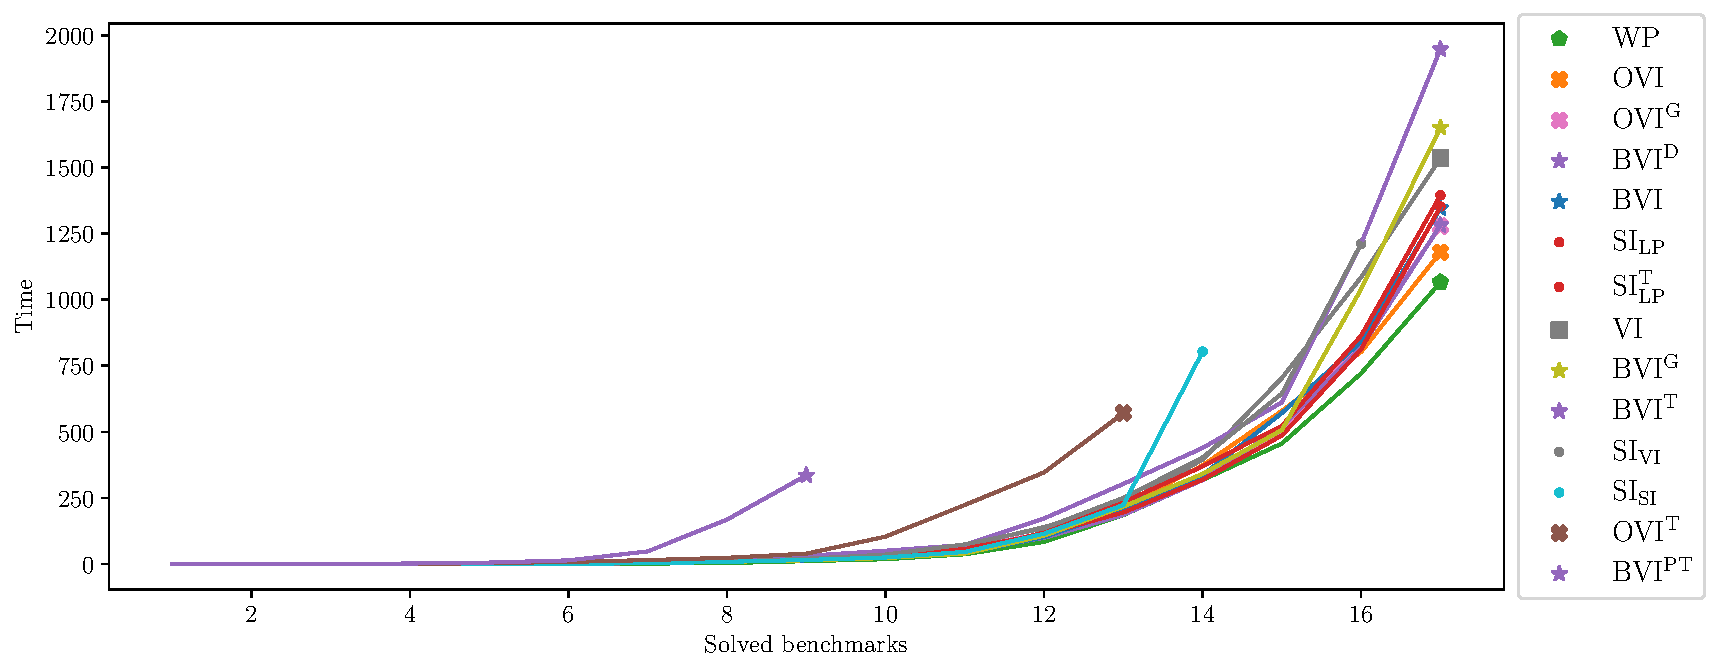
\includegraphics[width=1\textwidth]{figures/Real_AlgoPerformance.pdf} }}%
    \qquad
    \subfloat[\centering Accumulated algorithm performance overview on all randomly generated models.]{{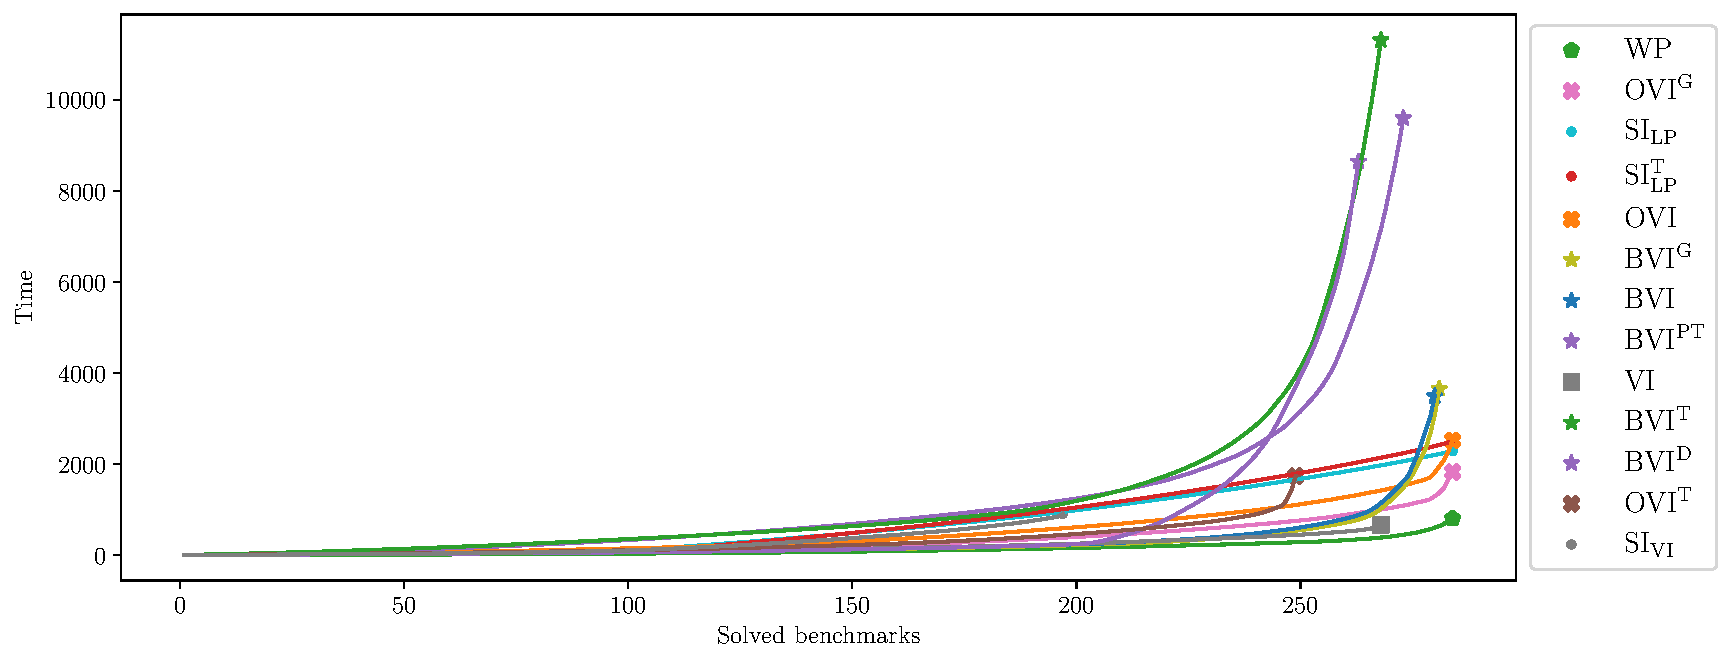
\includegraphics[width=1\textwidth]{figures/RandomRandom_AlgoPerformance.pdf} }}%
    \caption[Overview of Algorithm Performance]{
        A line plot providing an overview of the accumulated algorithm performance.
        The plot depicts the number of solved benchmarks (x-axis) and the time it took to solve them (y-axis). 
        For each algorithm, the benchmarks are sorted ascending by verification time. A line stops when no further benchmarks could be solved.
        Thus, the further to the bottom right a plot is, the better. Going right (solving benchmarks) is more relevant than having a low y-value.
        The legend on the right is sorted by the performance of the algorithms in descending order.
        }%
    \label{fig:AlgoPerformance}
\end{figure}

%For value-iteration-based algorithms, we provide the same graph with the number of iterations required to solve the models on the y-axis in Figure

We emphasize that since the times are displayed in accumulation and are very dependent of the models we use, 
the line plots only serve for rough overviews and provide insufficient information to compare algorithms that perform similar.

On one hand Figure \ref{fig:AlgoPerformance}(a) indicates that $\TOPAlg$ is the least performant algorithm, while $\BVID$, $\SISI$ and $\SI$ perform decent.
On the other hand, in Figure \ref{fig:AlgoPerformance}(b) $\TOPAlg$ is significantly better, while $\BVID$, $\SISI$ and $\SI$ are significantly worse than the other algorithms.
However, for both the real case studies and the randomly generated models $\WP$ and $\OVIG$ are the most performant algorithms. 
Furthermore, for both sets of models the topological optimization $\OVIT$ fails to solve significantly more models correctly than $\OVI$ or $\OVIG$.

We split our algorithm analysis into three subtopics: 
First, we compare the three value-iteration-based algorithms with guarantees $\OVI$, $\WP$, and $\BVI$. 
Then, we analyze the impact of the optimizations from Subsection \ref{subsec:optimizations} on their respective baseline algorithms.
Lastly, we investigate the performance of strategy-iteration-based algorithms in comparison to value-iteration-based algorithms.
For $\OVI$, $\WP$, $\BVI$ and their optimizations, we compare the number of iterations required to solve a model in addition to the time.
While time is practically more relevant, the number of iterations is independent of how sophisticated the implementation of the algorithm is.
\FloatBarrier

\subsection{$\BVI$ vs $\OVI$ vs $\WP$}
First, we compare bounded value iteration ($\BVI$), optimistic value iteration ($\OVI$) and widest path bounded value iteration ($\WP$) regarding their performance.
We observe in Figure \ref{fig:AlgoPerformance} that $\WP$ is the fastest approach for solving both randomly generated models and real case studies.
To see whether this is the case for all models or only when accumulating runtime, we provide a scatter plot in Figure \ref{fig:WPvsBVIvsOVI}.
The x-axis marks the time/iterations $\WP$ requires to solve a stochastic game, and the y-axis marks the respective time/iterations $\BVI$ or $\OVI$ needs.
The two thin lines next to the diagonal mark the case that $\WP$ is twice as fast as $\BVI$ / $\OVI$ or half as fast.

\begin{figure}[h!]
    \centering
    \subfloat[\centering Time required to solve a model]{{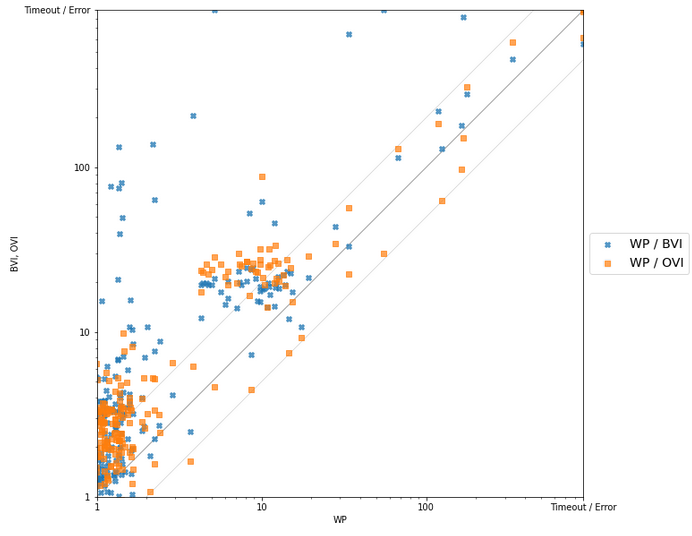
\includegraphics[width=.48\textwidth]{figures/WPvsBVIandOVIonAll.png} }}%
    \
    \subfloat[\centering Iterations required to solve a model]{{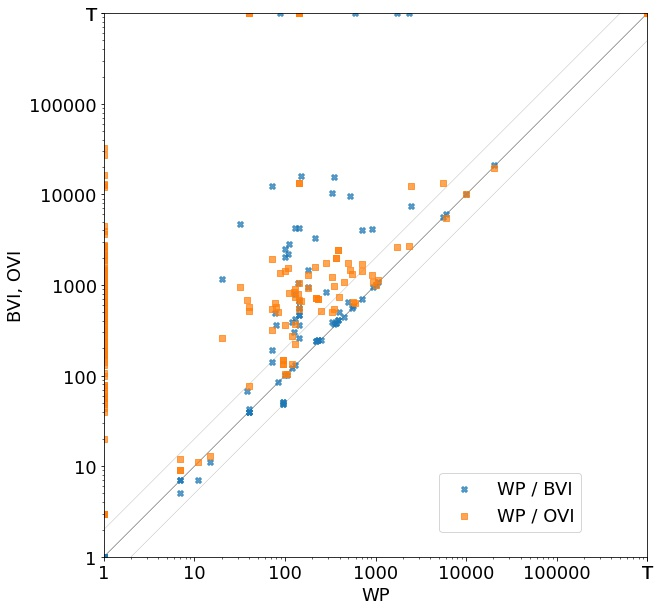
\includegraphics[width=.48\textwidth]{figures/WPvsBVIandOVIonAll_Iters.png} }}%
    \caption{$\WP$ compared to $\BVI$ and $\OVI$ on every model of datasets (i), (ii), and (iii) from Subsection \ref{subsec:casestudies}. See \ref{plot:performanceScatter} for a reference on how to read the plot.}%
    \label{fig:WPvsBVIvsOVI}%
    \end{figure}
\FloatBarrier

\subsubsection*{\underline{$\WP$}}
Regarding both time and iterations, although $\WP$ is the fastest algorithm when measuring accumulated runtime, it is neither consistently better nor worse than $\OVI$ and $\BVI$ on our benchmarks.
However, note that the difference between $\BVI$ and $\WP$ is how they solve end components. In our models, there are usually less than 3 MECs, and their size usually does not exceed 5 states.
Thus, we have created a dataset randomly using the RandomSCC guideline with 10 models and 10000 states each. Each model contains a large MEC with at least 9000 states.
While $\WP$ required per model no more than 30 seconds, $\OVI$ solved only 3 models with 5 to 9 minutes per model, and $\BVI$ solved none within a 15 minutes timeframe. 
Since $\WP$ is consistently one of the fastest algorithms and excels at solving MECs, we conclude that it is the best initial choice in case of doubt.

\subsubsection*{\underline{$\BVI$}}

Figure \ref{fig:BVIvsWPvsOVI} provides an overview of the time $\BVI$ requires to solve a model compared to $\OVI$ and $\WP$.
While both the accumulated runtime of Figure \ref{fig:AlgoPerformance} and Figure \ref{fig:BVIvsWPvsOVI}(a)
suggest that for more complicated models $\OVI$ and $\WP$ are faster than $\BVI$, 
Figure \ref{fig:BVIvsWPvsOVI}(b) shows that for large models $\BVI$ tends to be faster. 
However, we emphasize that this tendency may be due to a lack of a diverse dataset for large models.

\begin{figure}[h!]
    \centering
    \subfloat[\centering Time required to solve for all models from Subsection \ref{subsec:casestudies}]{{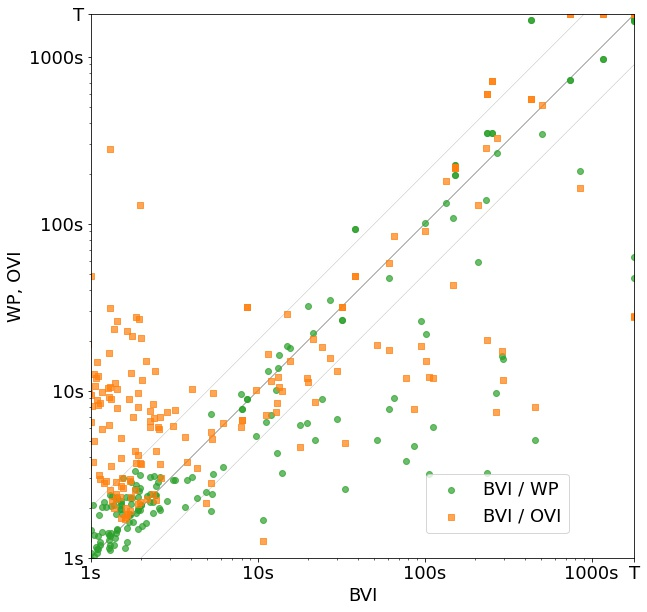
\includegraphics[width=.48\textwidth]{figures/BVIvsWPvsOVI.jpg} }}%
    \
    \subfloat[\centering Time required to solve for all large models as described in Subsection \ref{subsec:casestudies} (iv)]{{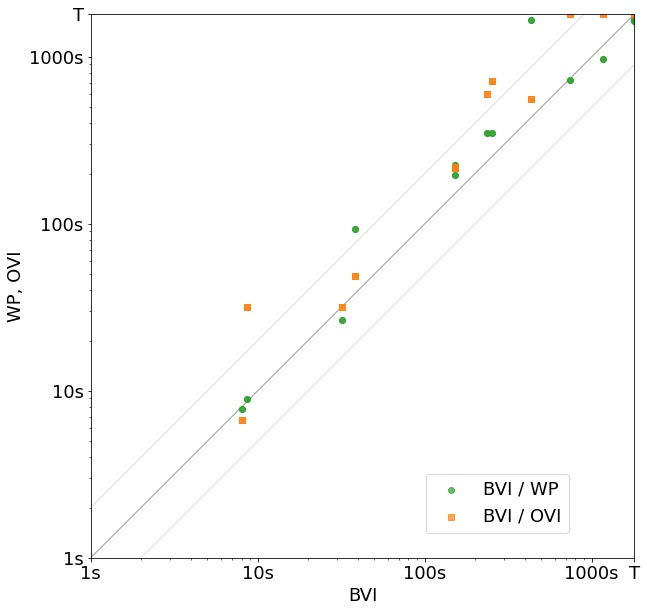
\includegraphics[width=.48\textwidth]{figures/BVIvsWPvsOVI_OnlyBig.jpg} }}%
    \caption{$\BVI$ compared to $\WP$ and $\OVI$. See \ref{plot:performanceScatter} for a reference on how to read the plot.}%
    \label{fig:BVIvsWPvsOVI}%
    \end{figure}
\FloatBarrier

We found that $\BVI$ usually requires fewer iterations than $\OVI$ to solve a model.
The reasons for that are explained in the following paragraph:

\subsubsection*{\underline{$\OVI$}}
$\OVI$ seems performant when looking at accumulated runtime and the scatter plot of Figure \ref{fig:WPvsBVIvsOVI}(a).
However, optimistic value iteration is a heuristic whose performance depends on never failing when guessing a bound.
We recall that whenever $\OVI$ guesses a bound that is neither an upper nor a lower bound, it halves its $\epsilon'$ and must continue iterating on the lower bound.
The next verification phase will only start once no states value changes by more than the new $\epsilon'$.
Thus, it is possible that the verification phase fails even though the value of each state is already very close to the required precision.
In that case, $\OVI$ will perform unnecessary extra iterations until it reaches $\epsilon'$ and verifies that $\OVI$ may indeed terminate.
We found that on every model where $\OVI$ performs as well as $\WP$ or $\BVI$ there was no verification phase that failed.
\textcolor{purple}{But pretty much all models required only one verification phase so what is the deal here? It is probably interesting to see how many jumps 
we had and how many verification phases failed}.
However, we expect that larger models may more likely contain subsets of states that may require multiple verification phases, 
but did not sufficiently investigate the behavior of $\OVI$ on arbitrary large models to validate this statement.

On the other hand, there are also conditions at which $\OVI$ is better than $\WP$ and $\BVI$.
While both $\WP$ and $\BVI$ require that both lower and upper bound converge, 
$\OVI$ can solve models easily where the lower bound converges quickly, but the upper bound does not.
However, we were unable to successfully correlate and model feature we track to fast lower bound convergence paired with slow upper bound convergence. 

Next, we evaluate the number of iterations optimistic value iteration needs. $\OVI$ generally requires more iterations than $\WP$ and $\BVI$. This is partly because of the extra iterations that may happen in $\OVI$ as mentioned, 
and partly because during verification phase only the upper bound is being iterated on. Meanwhile, in $\BVI$ both upper- and lower bound are updated per iteration.
Also, it is interesting to see that for about half of the models in Figure \ref{fig:WPvsBVIvsOVI} $\WP$ requires only 1 iteration whereas $\OVI$ requires many iterations to solve the model.
The red dots in Figure \ref{fig:OVIinstantCompute} visualize the value of the games where $\WP$ required only 1 iteration and $\OVI$ multiple,
while the green dots represent models where $\WP$ required also multiple iterations to solve the game.

\begin{figure}[h!]
    \centering
    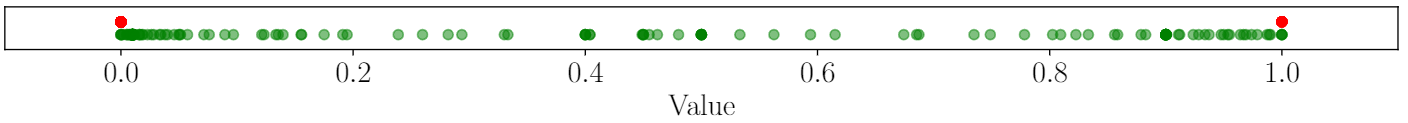
\includegraphics[width=1\textwidth]{figures/OVI_Bad_At_Computing_Instant_Values.png}
    \caption[$\OVI$ cannot instantly compute models]{
        A one dimensional scatter plot of when $\WP$ could solve a model in 1 iteration while $\OVI$ could not (red) 
        against where $\WP$ requires more than 1 iteration (green).
    }
    \label{fig:OVIinstantCompute}
\end{figure}
\FloatBarrier

Clearly, in some instances where a game has value 0 or 1, $\WP$ is able to identify its value in only 1 iteration while $\OVI$ cannot.
$\BVI$ is also capable of solving these models in 1 iteration.
In the runtime scatter plot of Figure \ref{fig:WPvsBVIvsOVI}, these models are mostly the cloud of orange dots in the lower left quadrant.
However, even if $\BVI$ and $\WP$ require only one iteration, they still require various seconds to perform this iteration, as Figure \ref{fig:BVI1IterationTime}.
The outliers that require more than 80 seconds to solve for $\BVI$ are variations of the real case study "Avoid the Observer" from \cite{cav20}.
\begin{figure}[h!]
    \centering
    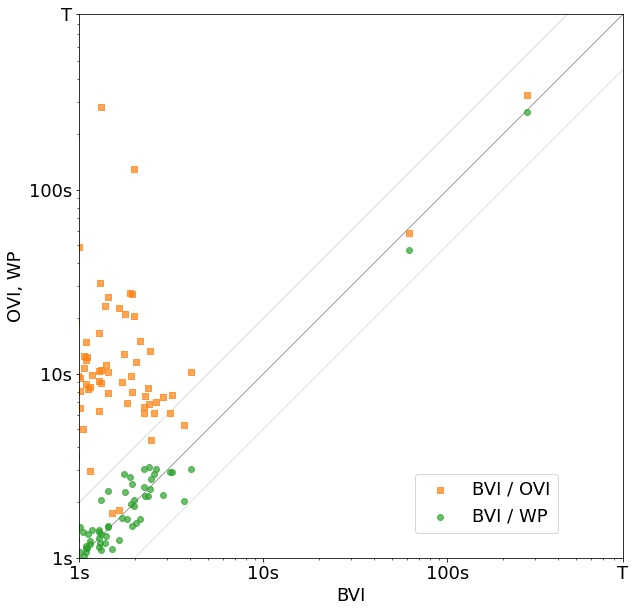
\includegraphics[width=0.4\textwidth]{figures/BVI_1_Iteration_vs_OVI.jpg}
    \caption[Time $\BVI$ requires solving models where it only needs one iteration]{
        A scatter plot of the time $\BVI$ requires solving models where $\BVI$ and $\WP$ require only one iteration to solve the model, 
        but $\OVI$ requires multiple iterations. 
    }
    \label{fig:BVI1IterationTime}
\end{figure}
\FloatBarrier

\subsection{Analyzing the optimizations}
After comparing the extensions for value iteration, we evaluate the impact of including optimizations like topological ordering or using the Gauss-Seidel optimization.
Figure \ref{fig:AlgoPerformance} indicates that optimizations introduced in Subsection \ref{subsec:optimizations} do not always improve the accumulated runtime. 
For example, while $\BVID$ is better than $\BVI$ in the real case studies, it is significantly worse on our randomly generated models.
To analyze the effect of the optimizations, we compare $\BVI$, $\OVI$, and $\LPSI$ with the optimizations that apply to them in scatter plots.
To each optimization, we provide a scatter plot with time required to solve the models, and one scatter plot with iterations required to solve the models.
For the iterations scatter plots we include only $\BVI$ and $\OVI$ since iterations in strategy iteration are not comparable to iterations in value iteration.

\subsubsection*{\underline{$\mathbf{Gauss-Seidel}$ for $\BVI$}:}
\begin{figure}[h!]
    \centering
    \subfloat[\centering Time required to solve a model]{{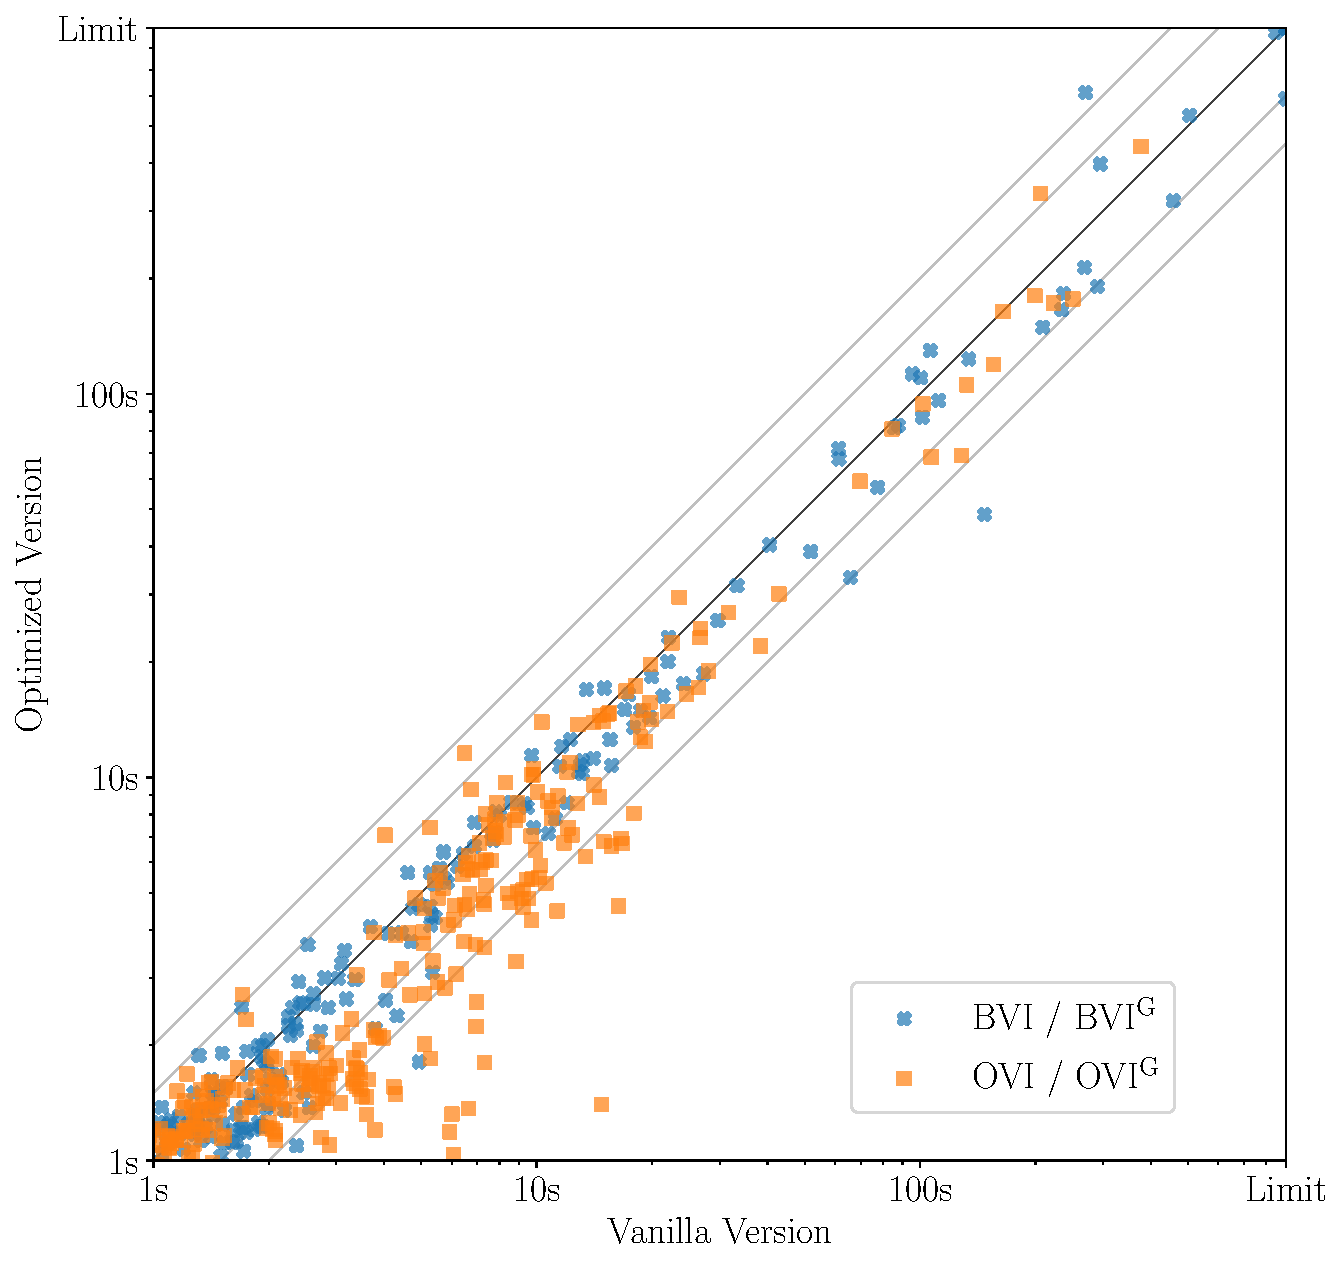
\includegraphics[width=.48\textwidth]{figures/Scatter_G.pdf} }}%
    \
    \subfloat[\centering Iterations required to solve a model]{{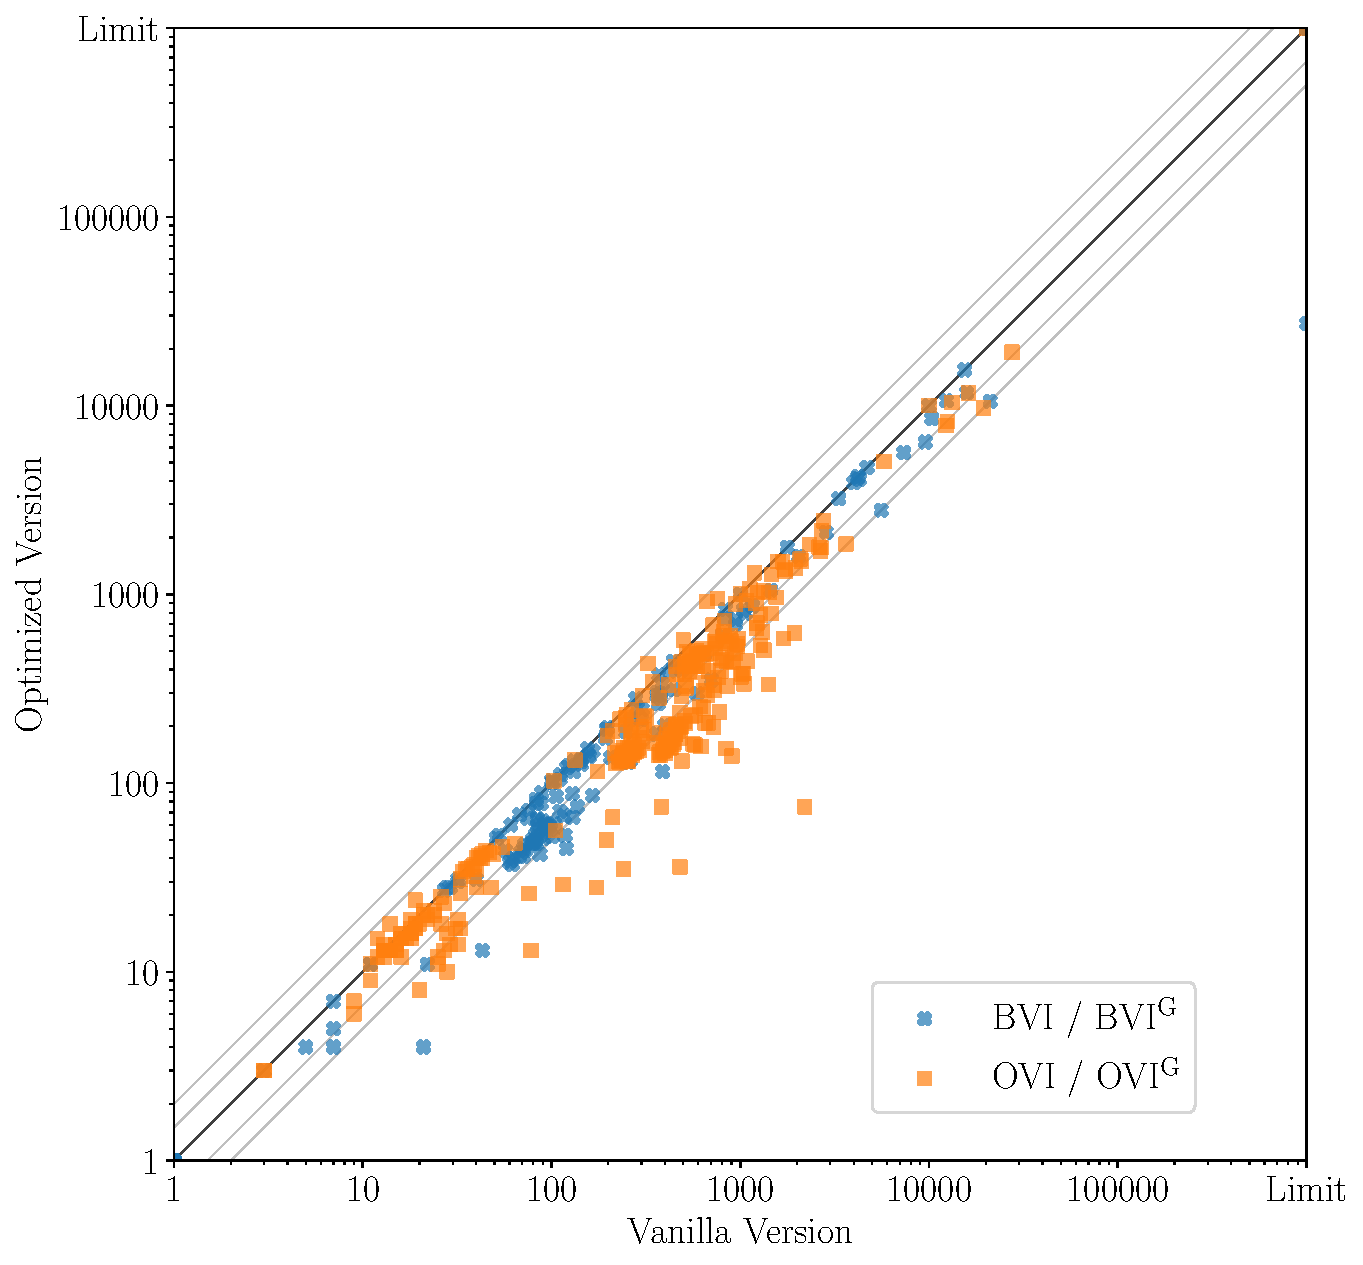
\includegraphics[width=.48\textwidth]{figures/Scatter_G_iters.pdf} }}%
    \caption{$\BVI$ and $\OVI$ compared to their Gauss-Seidel optimizations on every model of datasets (i), (ii), and (iii) from Subsection \ref{subsec:casestudies}}%
    \label{fig:Scatter_G}%
    \end{figure}

As Figure \ref{fig:Scatter_G} suggests, using the Gauss-Seidel optimization may reduce both the time and iterations required to solve a model by up to 4 times in most cases.
The Gauss-Seidel optimization is slower in some cases because the values are computed state by state to enable using already computed results.
The unoptimized version uses vector operations instead, which is faster sometimes.

In a few instances, the Gauss-Seidel optimization requires more iterations than the unoptimized version. 
This is because $\OVI$ and $\BVI$ may find different end components to deflate depending on whether Gauss-Seidel is used or not.
In some cases, the unoptimized version is able to find more favorable sets of end components and requires thus less iterations.
Changing the order of computation of the states for the Gauss-Seidel optimization by computing along a topological enumeration of the states did not
yield improvements in our experiments. 
\FloatBarrier 

\subsubsection*{\underline{$\mathbf{D}$ for $\BVI$}:}
\begin{figure}[h!]
    \centering
    \subfloat[\centering Time required to solve a model]{{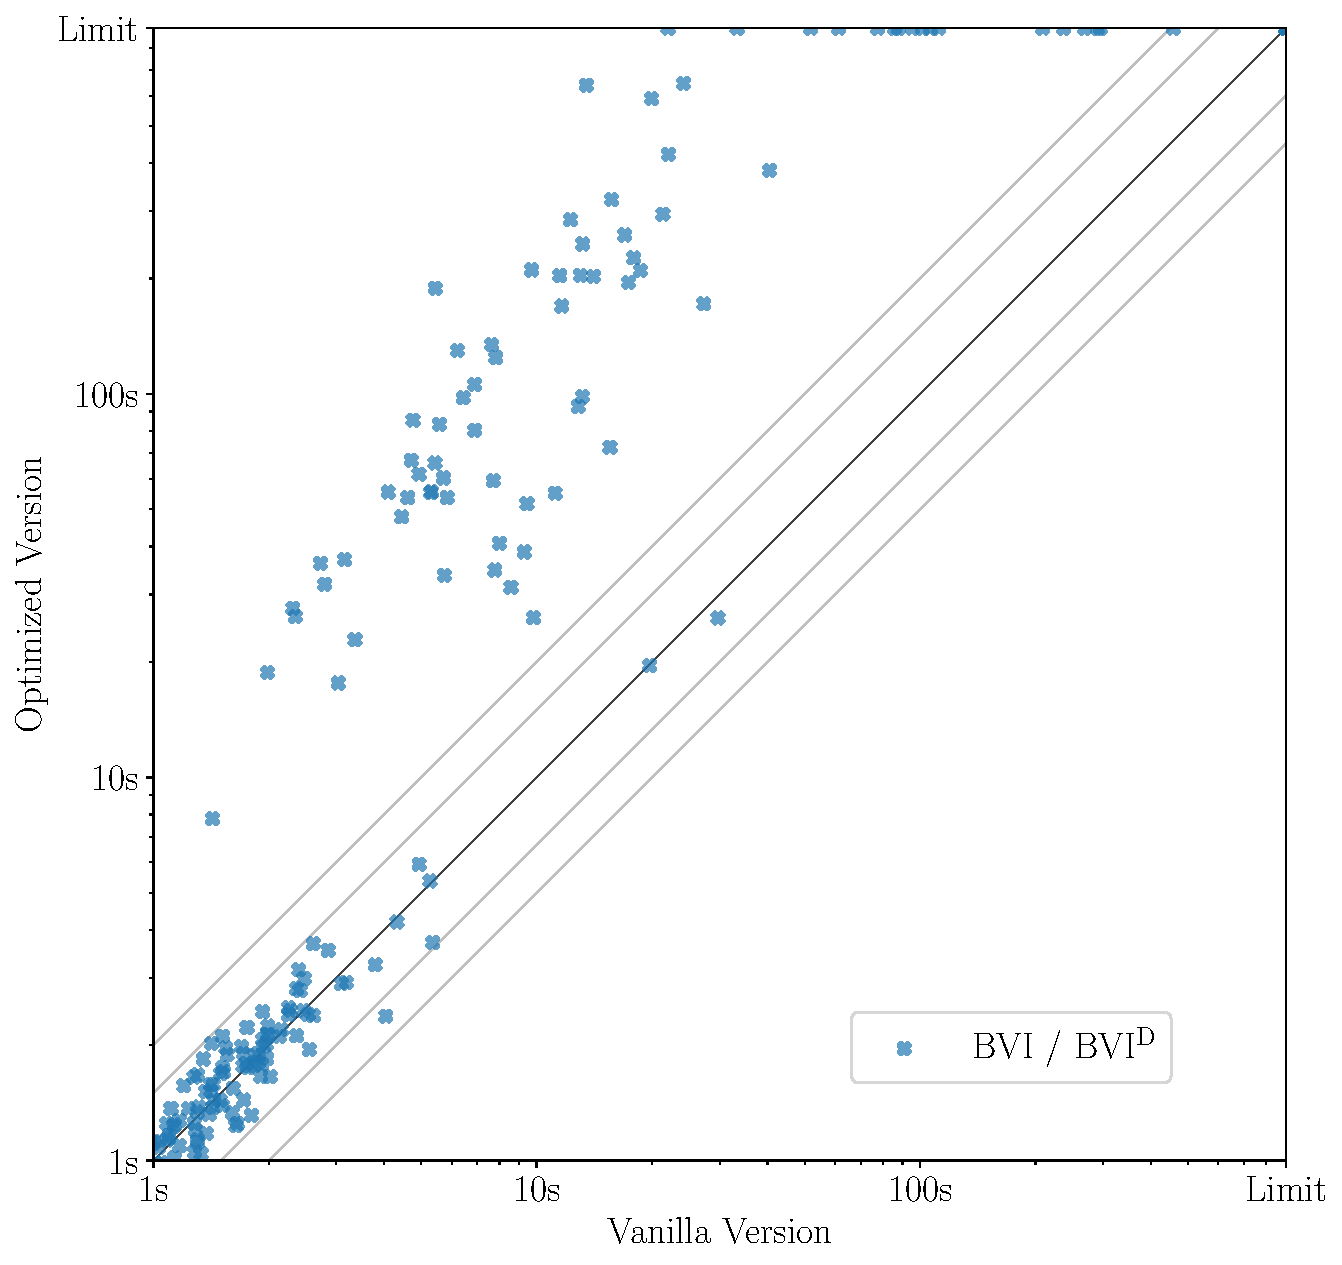
\includegraphics[width=.48\textwidth]{figures/Scatter_D.pdf} }}%
    \
    \subfloat[\centering Iterations required to solve a model]{{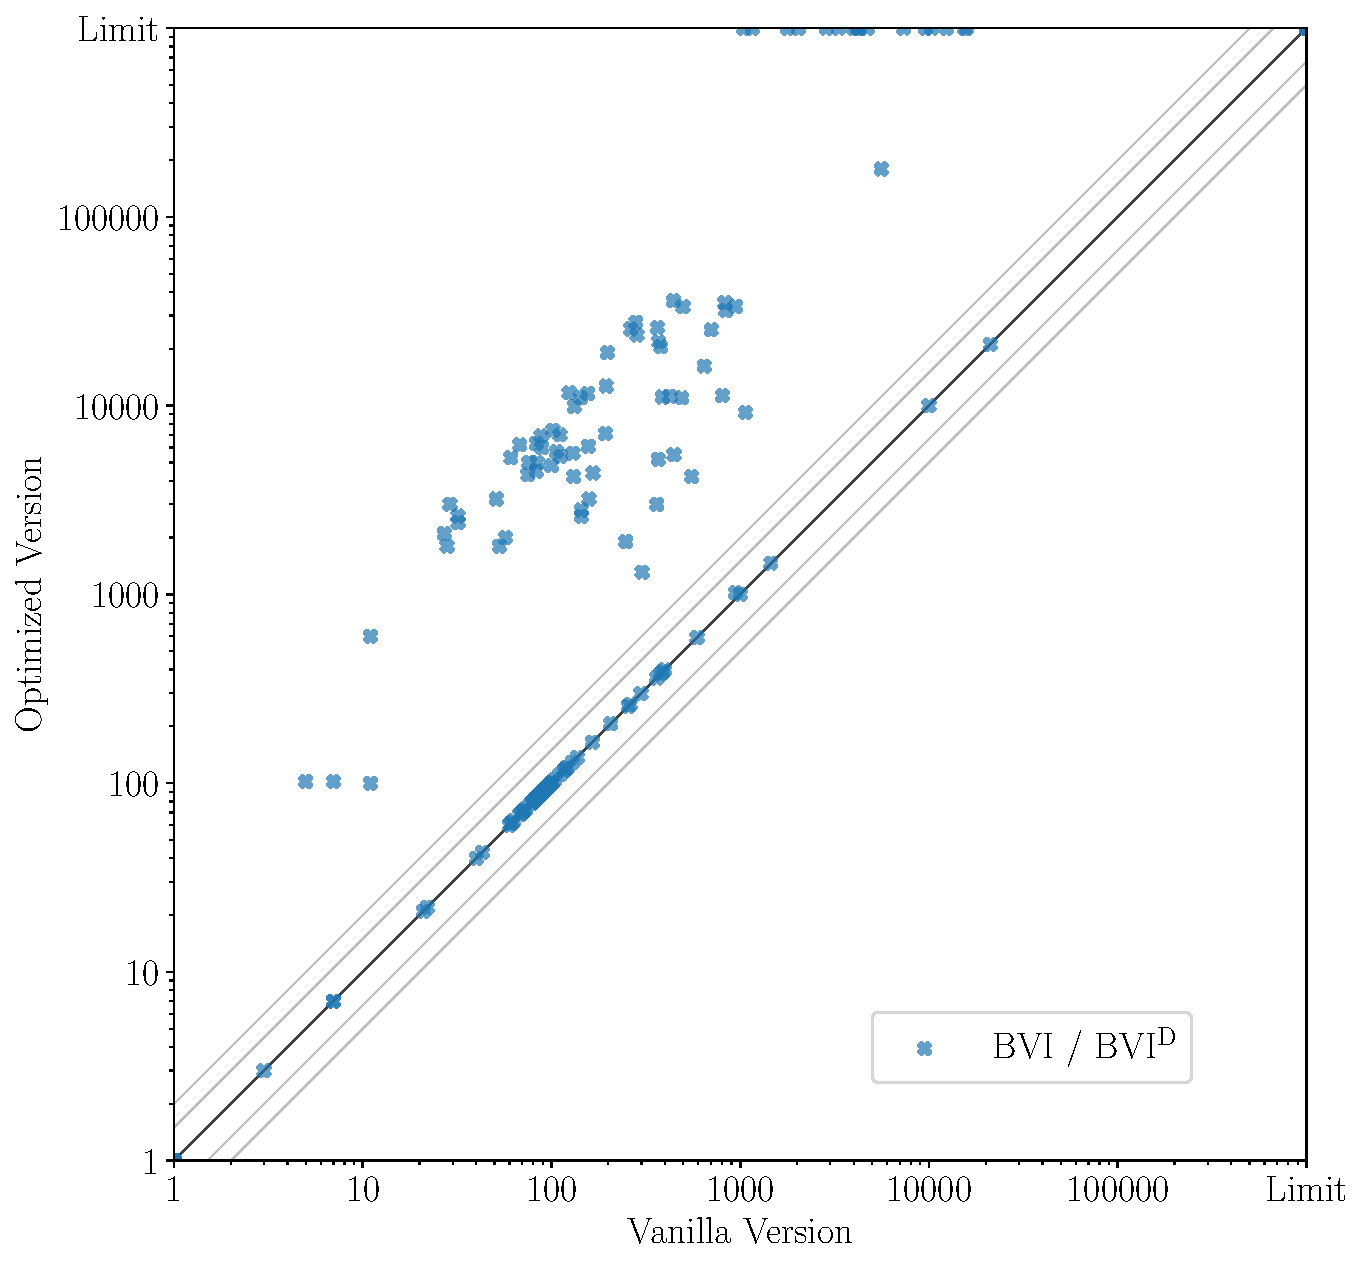
\includegraphics[width=.48\textwidth]{figures/Scatter_D_iters.pdf} }}%
    \caption{$\BVI$ compared to its optimization where deflating happens only every 100 iterations on every model of datasets (i), (ii), and (iii) from Subsection \ref{subsec:casestudies}}%
    \label{fig:Scatter_D}%
    \end{figure}
Figure \ref{fig:Scatter_D} clearly indicates that although $\BVID$ may solve sometimes models faster, 
for most of our models it could not compete with $\BVI$. 
Almost all models where $\BVI$ is more than twice as fast as $\BVID$ have at least three MECs.
Furthermore, almost all models where $\BVI$ and $\BVID$ require the same number of iterations have no end components.

\subsubsection*{\underline{$\mathbf{T}$ for $\BVI, \OVI$ and $\LPSI$}:} \label{subsubsec:topologicalOptim}
\begin{figure}
    \centering
    \subfloat[\centering Time required to solve a model]{{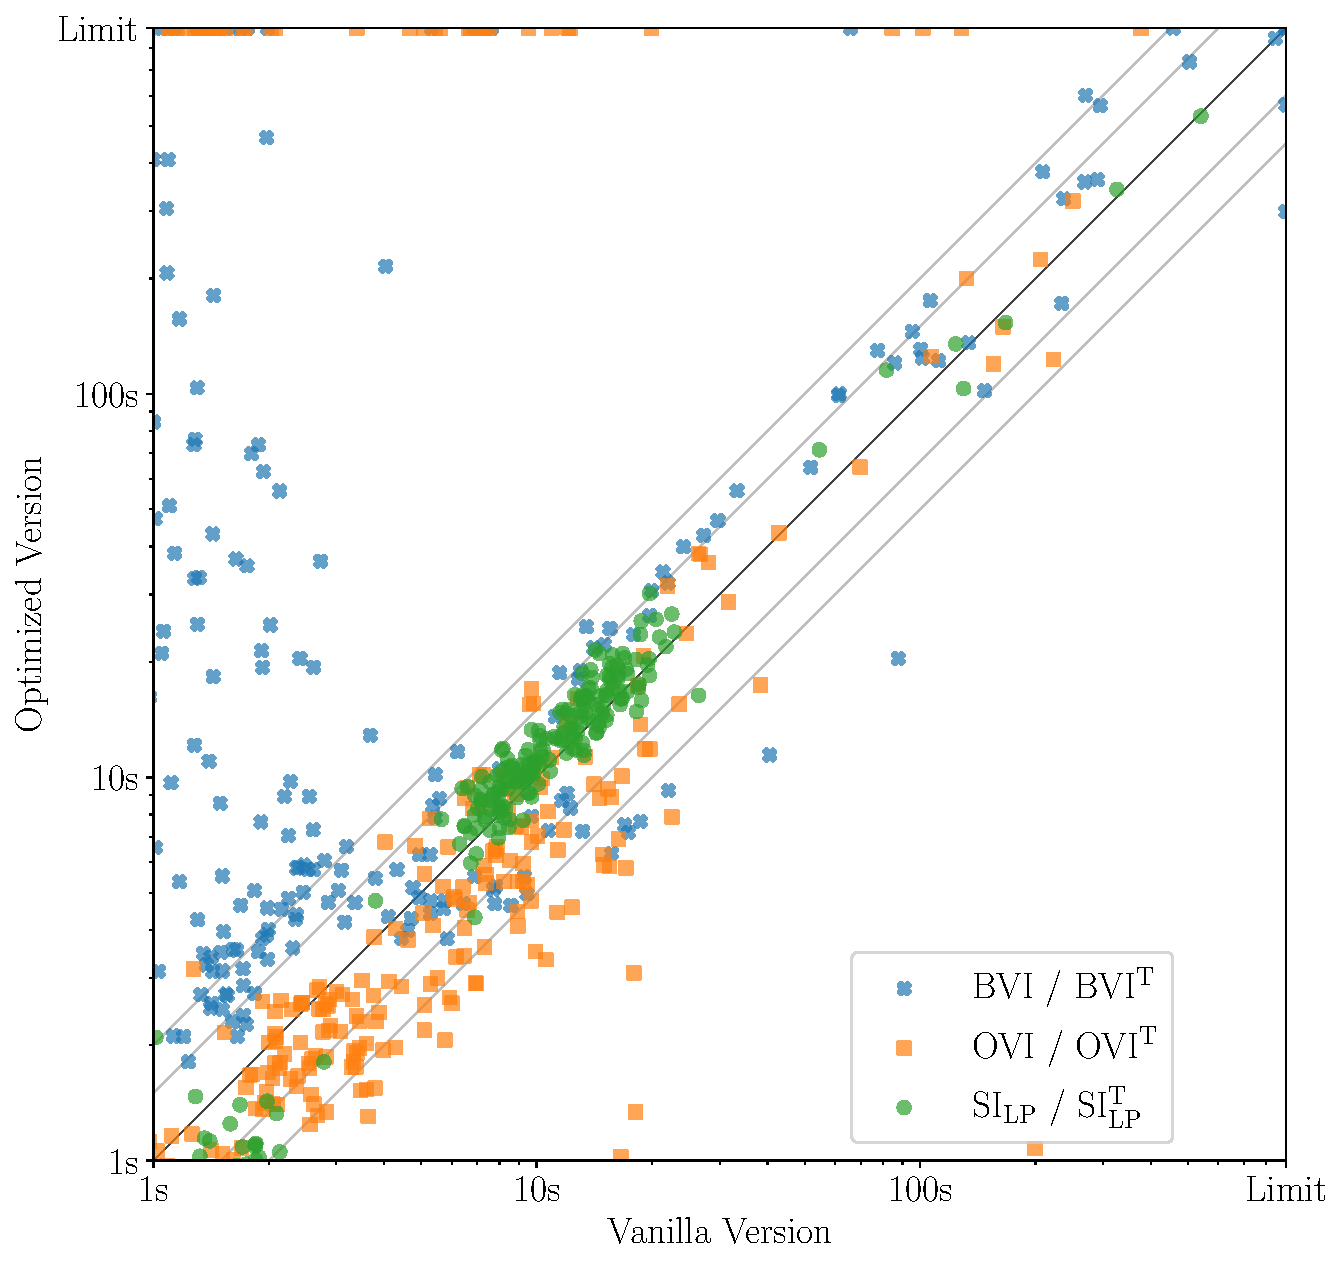
\includegraphics[width=.48\textwidth]{figures/Scatter_T.pdf} }}%
    \
    \subfloat[\centering Iterations required to solve a model]{{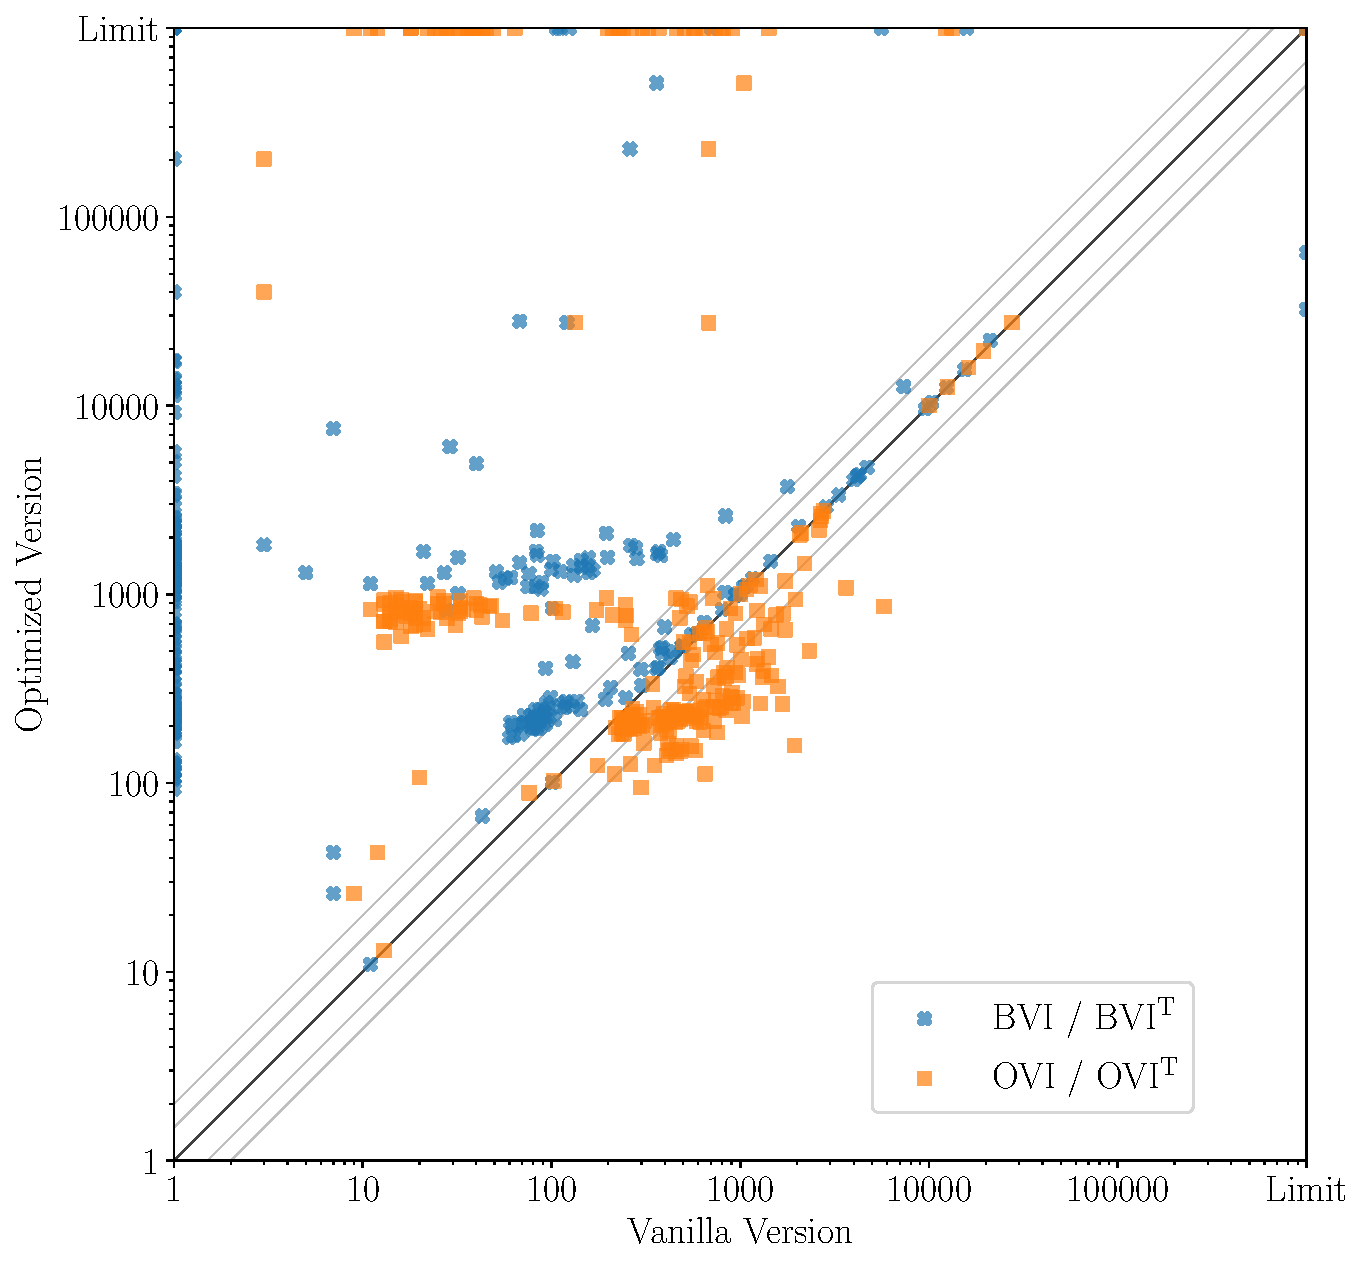
\includegraphics[width=.48\textwidth]{figures/Scatter_T_iters.pdf} }}%
    \caption{$\BVI$, $\OVI$ and $\LPSI$ compared to their topological optimizations on every model of datasets (i), (ii), and (iii) from Subsection \ref{subsec:casestudies}}%
    \label{fig:Scatter_T}%
    \end{figure}
As Figure \ref{fig:Scatter_T} displays, the topological optimization improves the runtime of $\OVI$ considerably. 
However, $\OVIT$ returns an incorrect value in around 10\% of all models. \textcolor{red}{Talk with Maxi about that}

From the strategy iteration variants, we use $\LPSI$ since it is the most performant variant.
For $\LPSI$, the topological optimization does neither in- nor decrease the performance of the algorithm considerably expect for case studies
like dice or MulMEC that have long chains of SCCs and favor topological algorithms.
Since $\TLPSI$ incurs very little overhead, we conclude that if in doubt use the topological variant.

Lastly, the topological optimization affects $\BVI$ usually negatively. As explained in \cite{gandalf}, 
chains of subsequent SCCs are harder to compute for $\BVIT$ because the values of the already computed SCCs are not exact, 
making it harder for the following SCCs to reach $\epsilon$-precision.
Another reason why $\BVI$ may be faster than its topological extension is because in one iteration every state in the whole graph is updated, 
while in the topological extension only states in the current SCC are updated.
An extreme example is a tree-like game with many states but only two levels: 
The initial state is the root and has a transition to every state, and every state is an SCC.
While the topological extension will solve every other SCC before solving the initial state, standard $\BVI$ may converge within significantly fewer iterations.
Note that this is not specific to $\BVIT$, but to any topological approach.
However, due to time limitations, we were unable to test this hypothesis.
\FloatBarrier

\subsubsection*{\underline{$\TOPAlg$}:}
\begin{figure}[h!]
    \centering
    \subfloat[\centering Time $\TOPAlg$ requires to solve a model of the datasets (i), (ii), and (iii) in comparison to $\BVI$ and $\BVIT$.]{{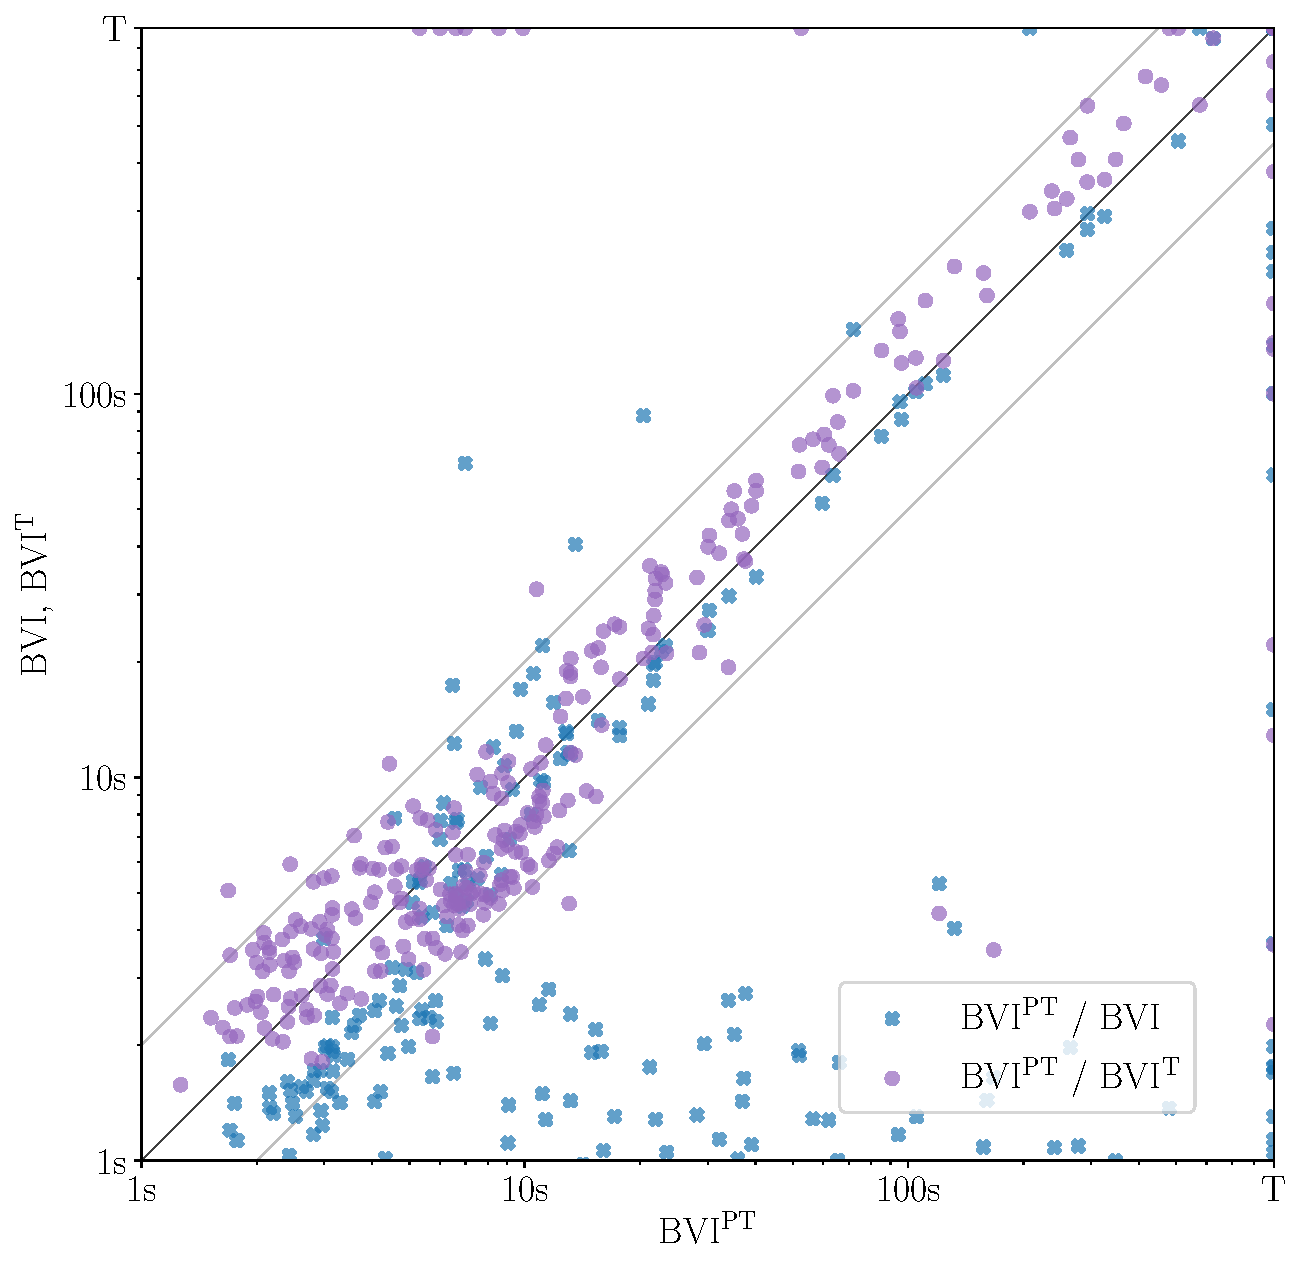
\includegraphics[width=.48\textwidth]{figures/TOPvsBVI_TBVI.pdf} }}%
    \
    \subfloat[\centering Time $\TOPAlg$ requires to solve a model of the dataset (iv) in comparison to $\BVI$.]{{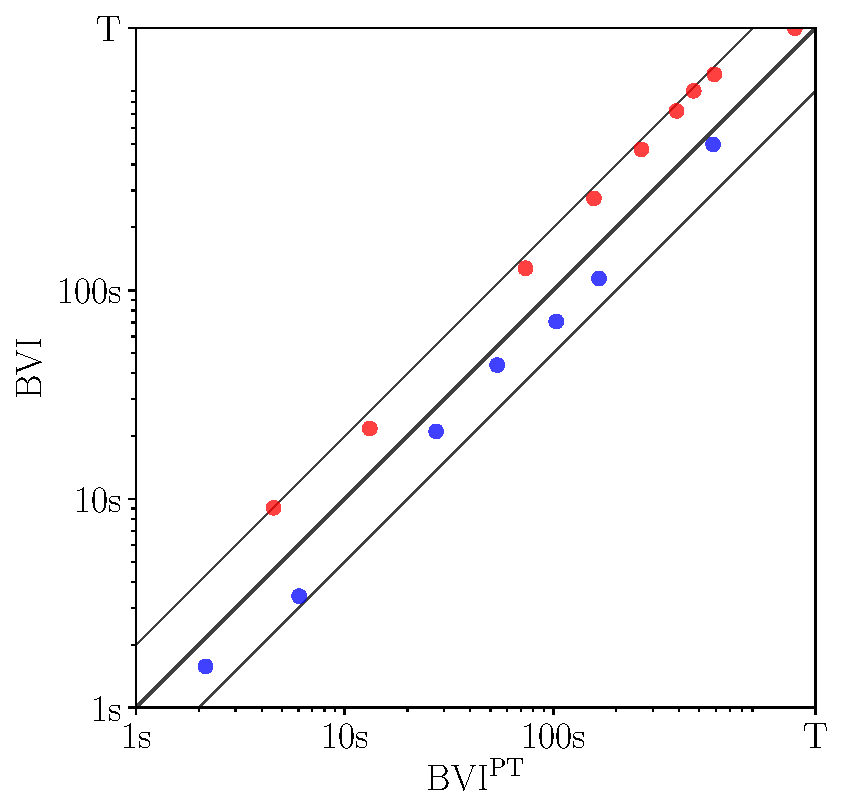
\includegraphics[width=.48\textwidth]{figures/bigConfBVIvsTOP.pdf} }}%
    \caption[$\TOPAlg$ compared to $\BVI$ with and without the topological optimization]{
        Two scatter plots of the time required for $\TOPAlg$ to solve a model in comparison to both $\BVI$ and $\BVIT$.
        For scatter plot (a), we have used real (i), handcrafted (ii) models, and randomly generated models (iii) as described in Subsection \ref{subsec:casestudies}.
        For scatter plot (b), we used the large, tree-like models (iv) as described in Subsection \ref{subsec:casestudies}. In the scatter plot (b),
        the blue dots are models where the whole state space consists of one large SCC, while models marked red dots have their state space divided into five equally large SCCs.
    }
    \label{fig:colorScatterBviTop}
\end{figure}

$\TOPAlg$ was introduced to solve the issues $\BVIT$ has with long chains of SCCs.
It successfully tackles the issues of $\BVIT$ and solves adversarial models for $\BVIT$ like the handcrafted model MulMEC fast.
While it is not generally better than $\BVIT$ on our benchmarks as Figure \ref{fig:colorScatterBviTop}(a) indicates, 
solving multiple SCCs is the only case where topological optimizations should be used. 
Thus, we conclude that $\TOPAlg$ makes $\BVIT$ obsolete.

When comparing $\TOPAlg$ to $\BVI$ it is clear that $\TOPAlg$ - like the topological optimization - impacts $\BVI$ usually negatively. 
$\TOPAlg$ is slower than $\BVI$ at solving many models where $\BVIT$ is also slower than $\BVI$.
Again, this might be due to the fact that $\BVI$ updates the whole state-space while topological variants must solve every SCC consecutively.
However, given a model that consists contains chains of large SCCs, $\TOPAlg$ is faster than standard bounded value iteration.
Figure \ref{fig:colorScatterBviTop}(b) indicates that if the model consists of one SCC, $\BVI$ is better than $\TOPAlg$ if there is only one SCC, 
but when the state space is divided into five equally sized SCCs, $\TOPAlg$ is more performant.

Lastly, note that $\TOPAlg$ may infer wrong strategies when computing the precise value for an SCC. 
In that case, $\TOPAlg$ throws an error and terminates. On our benchmark, in 5 out of 350 models this error was thrown.
\FloatBarrier

\subsection{Algorithms based on strategy iteration}
Although value iteration was regarded for a long time to be the most performant algorithm type for solving stochastic games, 
\cite{gandalf} showed that $\SI$ is a valid option, and that mathematical programming can be good sometimes.
Thus, in addition to $\SI$ we consider $\SISI$ and $\LPSI$ which do not use value iteration at all to solve stochastic games.

\subsubsection*{\underline{Strategy iteration with linear programming}}
On most of our models, $\LPSI$ yielded the best results alongside widest path bounded value iteration.
Since strategy iteration simply tries to make an informed decision on which strategy to pick and solves the underlying MDP, 
we have to inspect the algorithms we use to solve MDPs - for $\LPSI$ this is linear programming.

Linear programming scales worse than value iteration for huge models.
%As Figure \ref{fig:AlgoPerformanceBig} indicates, $\TLPSI$ and $\LPSI$ were slower to solve the models than $\OVI$, $\BVI$ and $\WP$.
%This is partly due to the LP solver running out of memory, which happened for models with SCC size of 10 million. 
On the large models used in Figure \ref{fig:colorScatterBviTop}(b), $\TLPSI$ is significantly less performant than $\TOPAlg$ independent of whether the model consisted of one or five SCCs.
If an SCC has at least 2 million states, $\TLPSI$ could not solve the corresponding model while $\TOPAlg$ could.
Additionally, as in \cite{gandalf}, we found that mathematical programming requires more memory than value iteration and thus is more prone to encounter 
out-of-memory exceptions for large models. 
In preliminary experiments we found that SCCs with more than 10 million states would run out of memory when using linear programming for MDPs and applying a memory limit of 36 GB.
Thus, we do not recommend using neither $\LPSI$ nor $\TLPSI$ on models with numerous states. 

%run several benchmarks on models with state size 10 million and varying SCC sizes. [Now enter Feature-Performance Scatter Plot] 
%The bigger the SCCs become, the slower $\TLPSI$ becomes. At a size of [...] per SCC, $\WP$ was faster than $\TLPSI$.}
However, $\TLPSI$ may be a good complementary solution approach in case a model is especially hard for value-iteration-based approaches.
The adversarial value iteration model hm from \cite{haddadmonmege} is solved by strategy iteration with linear programming within less than a second.

Lastly, in contrast to the other strategy iteration variants $\SISI$ and $\SI$, 
we could not find solid evidence that $\LPSI$ is negatively affected by increasing numbers of actions in a model.

%LP could likely be improved. At the moment, we do not even defslate but use MIP to encode the maximum-best-exit constraints. But this should maybe go into future work}

\subsubsection*{\underline{Strategy iteration with Markov chain solving}}
While $\SISI$ was unable to solve four out of 18 models in the real case studies, it failed at solving 179 out of 284 randomly generated models.
Figure \ref{fig:colorScatterSi}(a) indicates that this variant of strategy iteration is unable to solve models that have states with large numbers of actions.
This algorithm has to solve simple Markov chains instead of MDPs like $\LPSI$, and thus is less prone to out-of-memory errors. 
However, it has to solve significantly more linear equation systems.
We found that for the benchmark (iv) with large models $\SISI$ timed out whenever a model had more than 500000 states.

\subsubsection*{\underline{Strategy iteration with value iteration}}
While we confirm the findings of \cite{gandalf} that for the real models $\SI$ is comparable with $\BVI$, 
the accumulated runtime for the randomly generated models displayed in Figure \ref{fig:AlgoPerformance}(b) clearly shows that 
the models generated we generate are highly unfavorable for $\SI$.

\begin{figure}[h!]
    \centering
    \subfloat[\centering $\SISI$ compared to $\BVI$]{{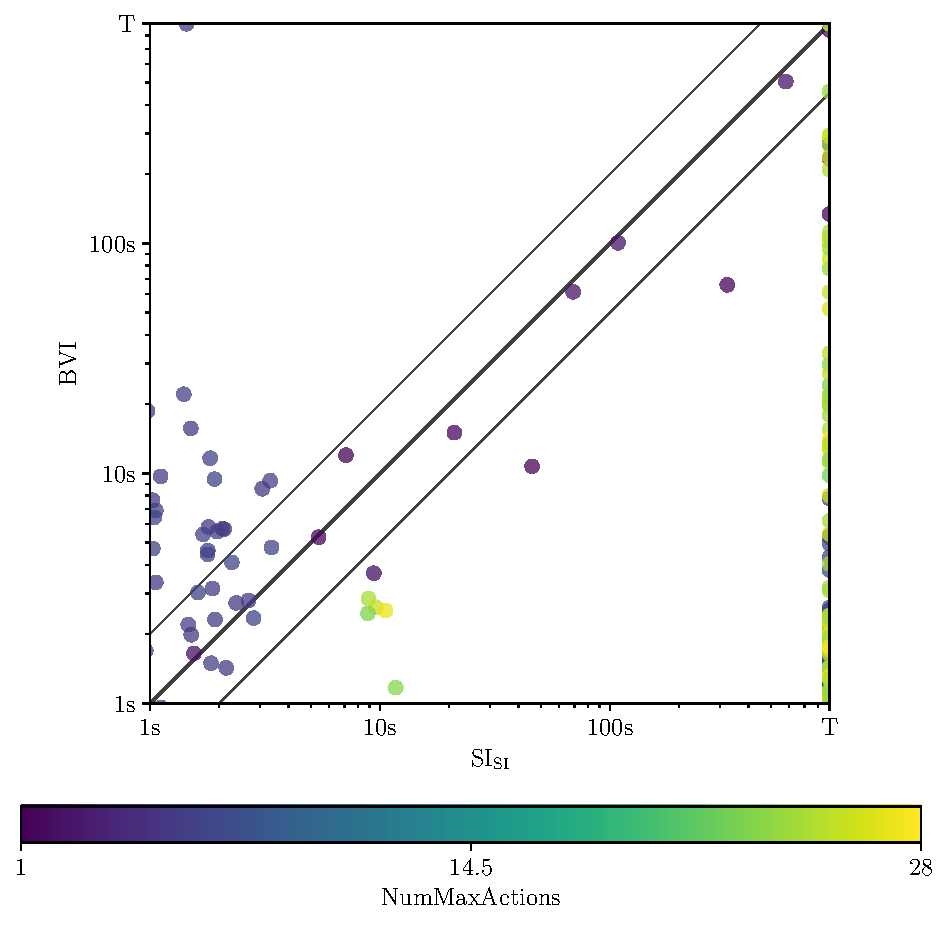
\includegraphics[width=.48\textwidth]{figures/SISI_colorscatter.pdf} }}%
    \subfloat[\centering $\SI$ compared to $\BVI$]{{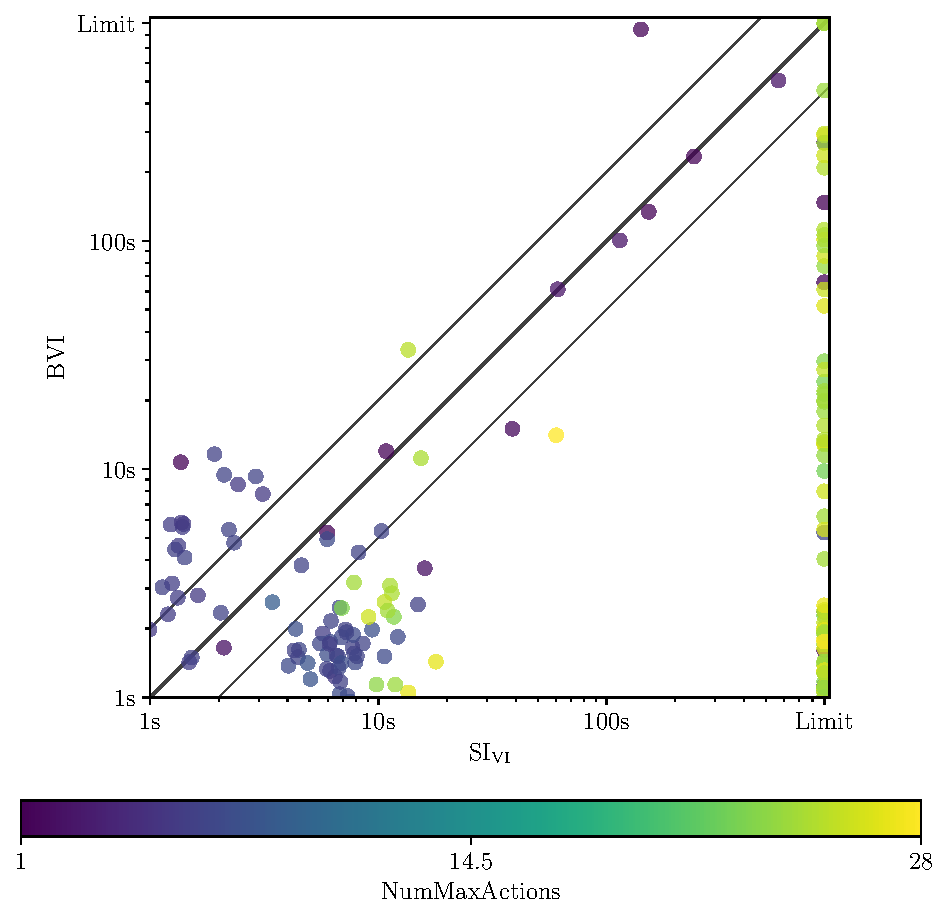
\includegraphics[width=.48\textwidth]{figures/colorScatter_SI_VI.pdf} }}%
    \caption[$\SI$ and $\SISI$ compared to $\BVI$ based on the maximal number of actions per state]{
        A scatter plot of time required for (a) $\SISI$ and (b) $\SI$ to solve a model from the datasets (i), (ii), (iii) as described in Subsection \ref{subsec:casestudies} 
        against the time $\BVI$ required.
        The dots are colored by the maximal number of actions per state.
        The more the color of a point goes towards yellow, the higher the maximal number of actions a state in the corresponding model has.
    }
    \label{fig:colorScatterSi}
\end{figure}
\FloatBarrier
This is most likely due to the higher number of actions per state of our generated models compared to the case studies.
As Figure \ref{fig:colorScatterSi}(b) suggests, if every state has up to 3 actions, $\SI$ and $\BVI$ perform similar.
However, as soon as there are states with more actions, $\SI$ is performing worse.
Another problem of strategy iteration with value iteration for MDPs is that, compared to $\LPSI$ for example, 
adversarial models for value iteration are also hard for $\SI$.
In addition to the approximately 100 models $\SI$ did not solve in time, 
5 models out of the 250 solved did not yield a correct result since using value iteration for MDP-solving does not guarantee correct results.